\documentclass[conference]{IEEEtran}
\IEEEoverridecommandlockouts
% The preceding line is only needed to identify funding in the first footnote. If that is unneeded, please comment it out.
\usepackage{cite}
\usepackage{amsmath,amssymb,amsfonts}
\usepackage{mathtools}
\usepackage{algpseudocode}
\usepackage{algorithm}
\usepackage{algorithmicx}
\usepackage{microtype}
\usepackage{float}
\usepackage{adjustbox}
\usepackage{booktabs,makecell,tabularx}
\usepackage{graphicx}
\usepackage{textcomp}
\usepackage{verbatim}
\usepackage{xcolor}
\usepackage{graphics} % for pdf, bitmapped graphics files
\usepackage{epsfig} % for postscript graphics files
\usepackage{mathptmx} % assumes new font selection scheme installed
\usepackage{multicol}
\usepackage{float}
\usepackage[english]{babel}
\usepackage[T1]{fontenc}
\usepackage{booktabs}
\restylefloat{table}
\def\BibTeX{{\rm B\kern-.05em{\sc i\kern-.025em b}\kern-.08em
    T\kern-.1667em\lower.7ex\hbox{E}\kern-.125emX}}
\begin{document}
\title{Quasi-Newton Methods Comparision using Ackley, Beale, Booth, Matyas, Rastrigin and RosenBrock Functions}
\author{
	\IEEEauthorblockN{Augusto Mathias Adams\IEEEauthorrefmark{1}, Caio Phillipe Mizerkowski\IEEEauthorrefmark{2}, Christian Piltz Araújo\IEEEauthorrefmark{3} and Vinicius Eduardo dos Reis\IEEEauthorrefmark{4}}\\
	\IEEEauthorblockA{\IEEEauthorrefmark{1}GRR20172143, augusto.adams@ufpr.br, \IEEEauthorrefmark{2}GRR20166403, caiomizerkowski@gmail.com,\\ \IEEEauthorrefmark{3}GRR20172197, christian0294@yahoo.com.br, \IEEEauthorrefmark{4}GRR20175957, eduardo.reis02@gmail.com}
}

\maketitle


\begin{abstract}
	This paper discusses briefly four popular algorithms to solve optimization/minimization problems, beloginging to Quasi-Newton class: \textit{Davidon–Fletcher–Powell} (DFP), \textit{Broyden–Fletcher–Goldfarb–Shanno} (BFGS), \textit{limited memory BFGS} and \textit{Levenberg-Marquardt Algorithm} (LMA). These algorithms are implemented in \textit{Python language}, version 3.10 and uses \textit{SymPy}, \textit{SciPy} and \textit{NumPy} libraries. One of them, \textit{BFGS}, is implemented natively on the  \textit{SciPy} library and the rest are implemented by hand to provide useful insights about the inner operation of the algorithms. The results are, however, very surprising with a few exceptions: when the initial solution is placed in a region near the global minimum, almost all algorithms converges very quickly and the convergence becomes unpredictable when the initial solution is placed randomly in the search space.
\end{abstract}

\begin{IEEEkeywords}
	Optimization Methods, Quasi-Newton, Second Order Optimization,  Non-linear Programming
\end{IEEEkeywords}

\section{Introduction}
\label{sec:introduction}

Quasi-Newton methods are methods used to find zeros or local maxima and minima of functions, as a viable alternative to Newton's method. They are generally used if the Jacobian or Hessian is not available or is too expensive to compute at each iteration. Strictly speaking, Newton's method requires the Jacobian to look for zeros, or the Hessian to find extrema, while quasi-Newton methods estimate the Jacobian or Hessian to perform such tasks.

In this paper, three popular alternatives of true \textit{Quasi-Newton} methods are evaluated to find function minima: \textit{Davidon–Fletcher–Powell} (DFP), \textit{Broyden–Fletcher–Goldfarb–Shanno} (BFGS) and \textit{limited memory BFGS} (LBFGS). The fourth method, the \textit{Levenberg-Marquardt Algorithm} (LMA) is a hybrid method that makes use of a weighting procedure between the steepest descent algorithm and Newton's method to obtain advantages from both methods.

The four methods were implemented using the Python language, based on the SciPy, NumPy and SimPy packages. The SciPy package already contains standard procedures for numerical optimization and uses the NumPy package for its internal operations. The SymPy package is used to assemble the test functions and is very convenient for differentiation of functions. The LBGFS, DFP and LMA methods, although they have native versions within the SciPy package, were implemented manually following SciPy conventions because the native versions do not support data collection of iterations and/or expect different parameters from the original proposal, such as LMA. The description of the manually implemented algorithms can be seen in the book Engineering Optimization by Singiresu Rao, Fifth Edition, except for LBFGS. The LBFGS algorithm was taken from GitHUB, in the url https://github.com/qkolj/L-BFGS/blob/master/L-BFGS.ipynb.

All algorithms were tested using the following parameters:

\begin{itemize}
	\item \textit{Number of initial Solutions:} 100
	\item \textit{Máximum Iterations:} 4000
	\item \textit{Tolerance (Convergence Criterion): } $1 \times 10^{-9}$
\end{itemize}

The initial solutions of all function were taken near the global minimum to avoid wrong convergence to a local minimum, since these algorithms don't differentiate a local minimum from a global minimum. It is assumed that the global minimum is a \textit{strong global minimum}, that is, a unique minimal point. For LMA, it is assumed that the initial step is fixed and does not take in consideration any information about the function/problem. All algorithms are unsconstrained and, while the initial solution is probably near the optimal solution, there's much room for divergence.

The algorithms were evaluated using the folowing criteria:

\begin{itemize}
	\item \textit{Convergence: } the convergence of an algorithm is classified as good, por and divergence.
	\subitem \textit{Good convergence: } the final solution is really near the optimal solution within the max iterations;
	\subitem \textit{Poor convergence: } the final solution is far from the optimal solution for any reason;
	\subitem \textit{Divergence: }  the final solution is out of the funtion's search space;
	\item \textit{Statistical Parameters about the solutions:} Mean and Median of the solutions are analysed to provide insights about the algorithms;
	\item Iterations to converge, function evaluations and function values.
\end{itemize}

\section{2D Function versions}
\label{functions2D}

\subsection{Ackley Function}
\label{ackley2D}

\subsubsection{Convergence Analysis}
\label{convergenceackley2D}


The convergence report for the Ackley Function is shown in Table~\ref{convergence:ackley}:

\begin{table}[H]
\centering
\caption{Convergence Report For Ackley Function}
\label{convergence:ackley}
\begin{tabular}{lrrrr}
\toprule
 Alg. &  Good &  Poor &  Diver. &  Total \\
\midrule
  dfp &   100 &     0 &       0 &    100 \\
 bfgs &   100 &     0 &       0 &    100 \\
lbfgs &   100 &     0 &       0 &    100 \\
  lma &   100 &     0 &       0 &    100 \\
\bottomrule
\end{tabular}
\end{table}

All algorithms converged 100 times, using 100 different initial solutions,
for a constrained search space of .$[-0.05, 0.05]$. This search space is around
the optimal solution to avoid wrong convergence to a local minimum.



\subsubsection{Statistical Analysis of The Solutions}
\label{statisticalanalysisackley2D}

The minimal. maximal, mean and median values of the solutions are shown in Table~\ref{function_values:ackley}:

\begin{table}[H]
\centering
\caption{Statistical Information about function values For Ackley Function}
\label{function_values:ackley}
\begin{tabular}{lrrrr}
\toprule
 Alg. &  Min &  Max &  Mean &  Median \\
\midrule
  dfp & 0.00 & 0.00 &  0.00 &    0.00 \\
 bfgs & 0.00 & 0.00 &  0.00 &    0.00 \\
lbfgs & 0.00 & 0.00 &  0.00 &    0.00 \\
  lma & 0.00 & 0.00 &  0.00 &    0.00 \\
\bottomrule
\end{tabular}
\end{table}

The values again are rounded. The matter is the mdian value: it informs us the result that
we are like to obtain when running any algorithm to solve for minimum. As it seems, for all
algorithms is expected to find the minimun of Ackley Function.


\subsubsection{Best Fits}
\label{bestfitsackley2D}

The best solutions of all algorithms for Ackley Function, obtained using the minimal
distance of the solution, are shown in Table~\ref{solutions:ackley}:

\begin{table}[H]
\centering
\caption{Best Fits For Ackley Function}
\label{solutions:ackley}
\begin{tabular}{llrrr}
\toprule
 Alg. &    Sol. &  Iter. &  F. Eval &  F. Value \\
\midrule
  dfp & $S_{1}$ &     36 &      108 &      0.00 \\
 bfgs & $S_{2}$ &     42 &      129 &      0.00 \\
lbfgs & $S_{3}$ &     37 &      389 &      0.00 \\
  lma & $S_{4}$ &     38 &      320 &      0.00 \\
\bottomrule
\end{tabular}
\end{table}

The Ackley function has a narrow space around the optimal solution and,
altough specially LMA is of rapid convergence, it iterated 38 times to find
the optimal value, probably because it walked around the solution
before reach it. All algorithms were very slow to converge and the most expensive
are LMA and LBFGS.

Altough the column F. Value points to the the same value, this is a rounded value
and the real values are os order $10^{-22} \approx 10^{-14}$.


The best solutions of all algorithms for Ackley Function, indicated as
$S_{1}$, $S_{2}$, $S_{3}$ and $S_{4}$ in Table~\ref{solutions:ackley}, are shown
in Table~\ref{detailedsolutions:ackley}:

\begin{table}[H]
\centering
\caption{Detailed Solutions For Ackley Function}
\label{detailedsolutions:ackley}
\begin{tabular}{lrrrr}
\toprule
 Coord. &  $S_{1}$ &  $S_{2}$ &  $S_{3}$ &  $S_{4}$ \\
\midrule
$x_{1}$ &    -0.00 &     0.00 &     0.00 &     0.00 \\
$x_{2}$ &    -0.00 &     0.00 &     0.00 &     0.00 \\
\bottomrule
\end{tabular}
\end{table}

The Table~\ref{detailedsolutions:ackley} shows the same solution to all algorithms, because the values are so small
and were rounded to fit on the Table. The differences of the optimal point are of order $10^{-14}$ to $10^{-22}$,
for the LMA, DFP, LBFGS and BFGS algorithms, respectively.


\subsubsection{Isolines and Convergence line}
\label{isolinesackley2D}

The isolines of Ackley Function and convergence lines for all algorithms are shown in Figure~\ref{fig:ackley}:\begin{figure}[H]
\centering
\caption{Isolines and convergence line for Ackley Function}
\label{fig:ackley}
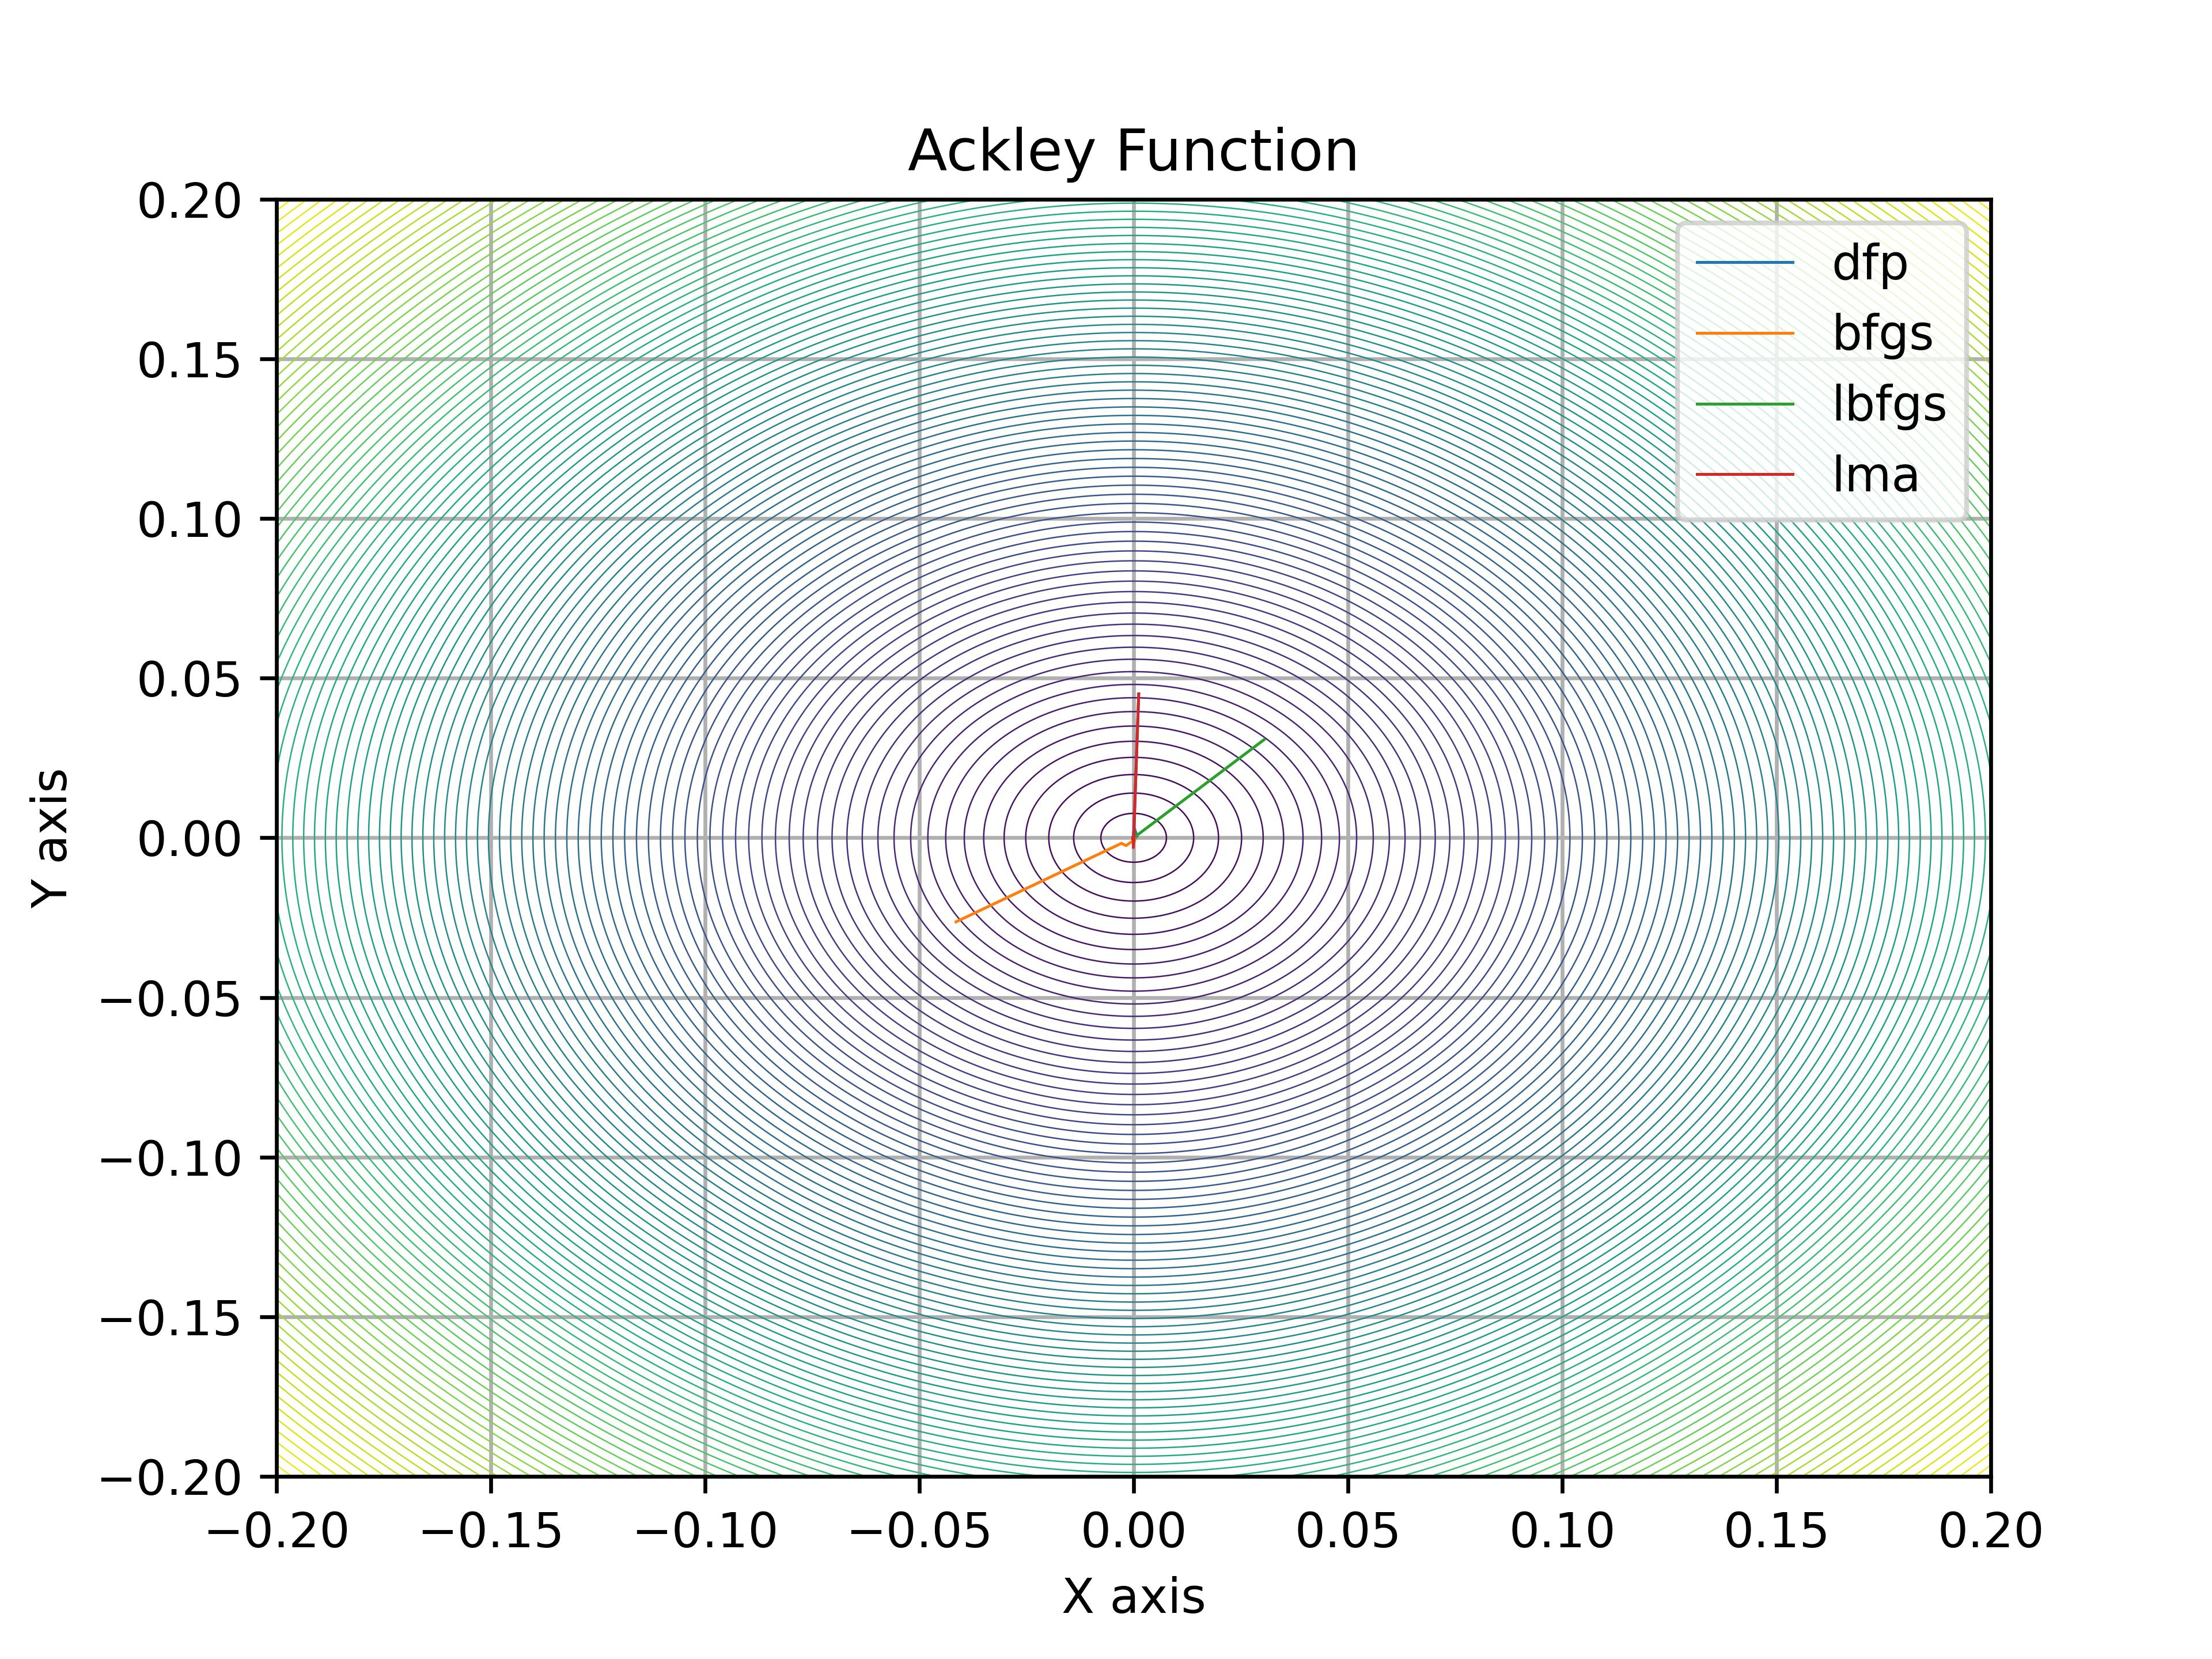
\includegraphics[scale=0.5]{images/ackley.jpg}
\end{figure}
The isolines for Ackley Function shows that there are at least 4 pitfalls near ther optimal solution, so, the search space needs to be reduced to \$[-0.05, 0.05]\$ to avoid wrong convergence. All the algorithms converges quite smoothly following a straight line\subsection{Beale Function}
\label{beale2D}

\subsubsection{Convergence Analysis}
\label{convergencebeale2D}


The convergence report for the Beale Function is shown in Table~\ref{convergence:beale}:

\begin{table}[H]
\centering
\caption{Convergence Report For Beale Function}
\label{convergence:beale}
\begin{tabular}{lrrrr}
\toprule
 Alg. &  Good &  Poor &  Diver. &  Total \\
\midrule
  dfp &    53 &    25 &      22 &    100 \\
 bfgs &    75 &     0 &      25 &    100 \\
lbfgs &    80 &     0 &      20 &    100 \\
  lma &    42 &    37 &      21 &    100 \\
\bottomrule
\end{tabular}
\end{table}

The Table~\ref{convergence:beale} show that not any algorithm
is capable to solve any problem. LMA had the worst performance
in good convergence, followed by DFP, BGFS and LBGFS. LBFGS has
a performance of 80\% in convergence.


\subsubsection{Statistical Analysis of The Solutions}
\label{statisticalanalysisbeale2D}

The minimal. maximal, mean and median values of the solutions are shown in Table~\ref{function_values:beale}:

\begin{table}[H]
\centering
\caption{Statistical Information about function values For Beale Function}
\label{function_values:beale}
\begin{tabular}{lrrrr}
\toprule
 Alg. &  Min &   Max &  Mean &  Median \\
\midrule
  dfp & 0.00 &  3.84 &  0.27 &    0.00 \\
 bfgs & 0.00 &  0.45 &  0.11 &    0.00 \\
lbfgs & 0.00 &  7.31 &  0.36 &    0.00 \\
  lma & 0.00 & 14.20 &  5.35 &    0.45 \\
\bottomrule
\end{tabular}
\end{table}

LMA again had the worst performance. It is the only algorithm that, altiugh has some solutions in
poor convergence, that has a median greater than zero. LBFGS and DFP seems quite radical in terms
of convergence, while having a median of zero its mean values are greater than zero an its maximal
value are noticeable. The larger mean value of LMA reinforces the notion of divergence in this case
and signifies that the algorithm don't fit very well for BEale Fnction minimum.


\subsubsection{Best Fits}
\label{bestfitsbeale2D}

The best solutions of all algorithms for Beale Function, obtained using the minimal
distance of the solution, are shown in Table~\ref{solutions:beale}:

\begin{table}[H]
\centering
\caption{Best Fits For Beale Function}
\label{solutions:beale}
\begin{tabular}{llrrr}
\toprule
 Alg. &    Sol. &  Iter. &  F. Eval &  F. Value \\
\midrule
  dfp & $S_{1}$ &      8 &       10 &      0.00 \\
 bfgs & $S_{2}$ &     15 &       18 &      0.00 \\
lbfgs & $S_{3}$ &     14 &       50 &      0.00 \\
  lma & $S_{4}$ &     12 &       13 &      0.00 \\
\bottomrule
\end{tabular}
\end{table}

The Beale function has a very large search space around the optimal solution and
it had a reasonable number of iterations for each algorithm. The DFP method, superseeded by BFGS,
is surprisingly rapid to find the solution. The LMA, known to be fast, had a reasonable performance.
BFGS/LBFGS performed as expected.

Altough the column F. Value points to the the same value, this is a rounded value
and the real values are os order $10^{-22} \approx 10^{-14}$.


The best solutions of all algorithms for Beale Function, indicated as
$S_{1}$, $S_{2}$, $S_{3}$ and $S_{4}$ in Table~\ref{solutions:beale}, are shown
in Table~\ref{detailedsolutions:beale}:

\begin{table}[H]
\centering
\caption{Detailed Solutions For Beale Function}
\label{detailedsolutions:beale}
\begin{tabular}{lrrrr}
\toprule
 Coord. &  $S_{1}$ &  $S_{2}$ &  $S_{3}$ &  $S_{4}$ \\
\midrule
$x_{1}$ &     3.00 &     3.00 &     3.00 &     3.00 \\
$x_{2}$ &     0.50 &     0.50 &     0.50 &     0.50 \\
\bottomrule
\end{tabular}
\end{table}

The optimal solution for Beale Function is $[3, 0.5]$ and the rounded values
of Table~\ref{detailedsolutions:beale} points to the same value. The error of
these values are of order $10^{-13}$ os less.



\subsubsection{Isolines and Convergence line}
\label{isolinesbeale2D}

The isolines of Beale Function and convergence lines for all algorithms are shown i Figure~\ref{fig:beale}:\begin{figure}[H]
\centering
\caption{Isolines and convergence line for Beale Function}
\label{fig:beale}
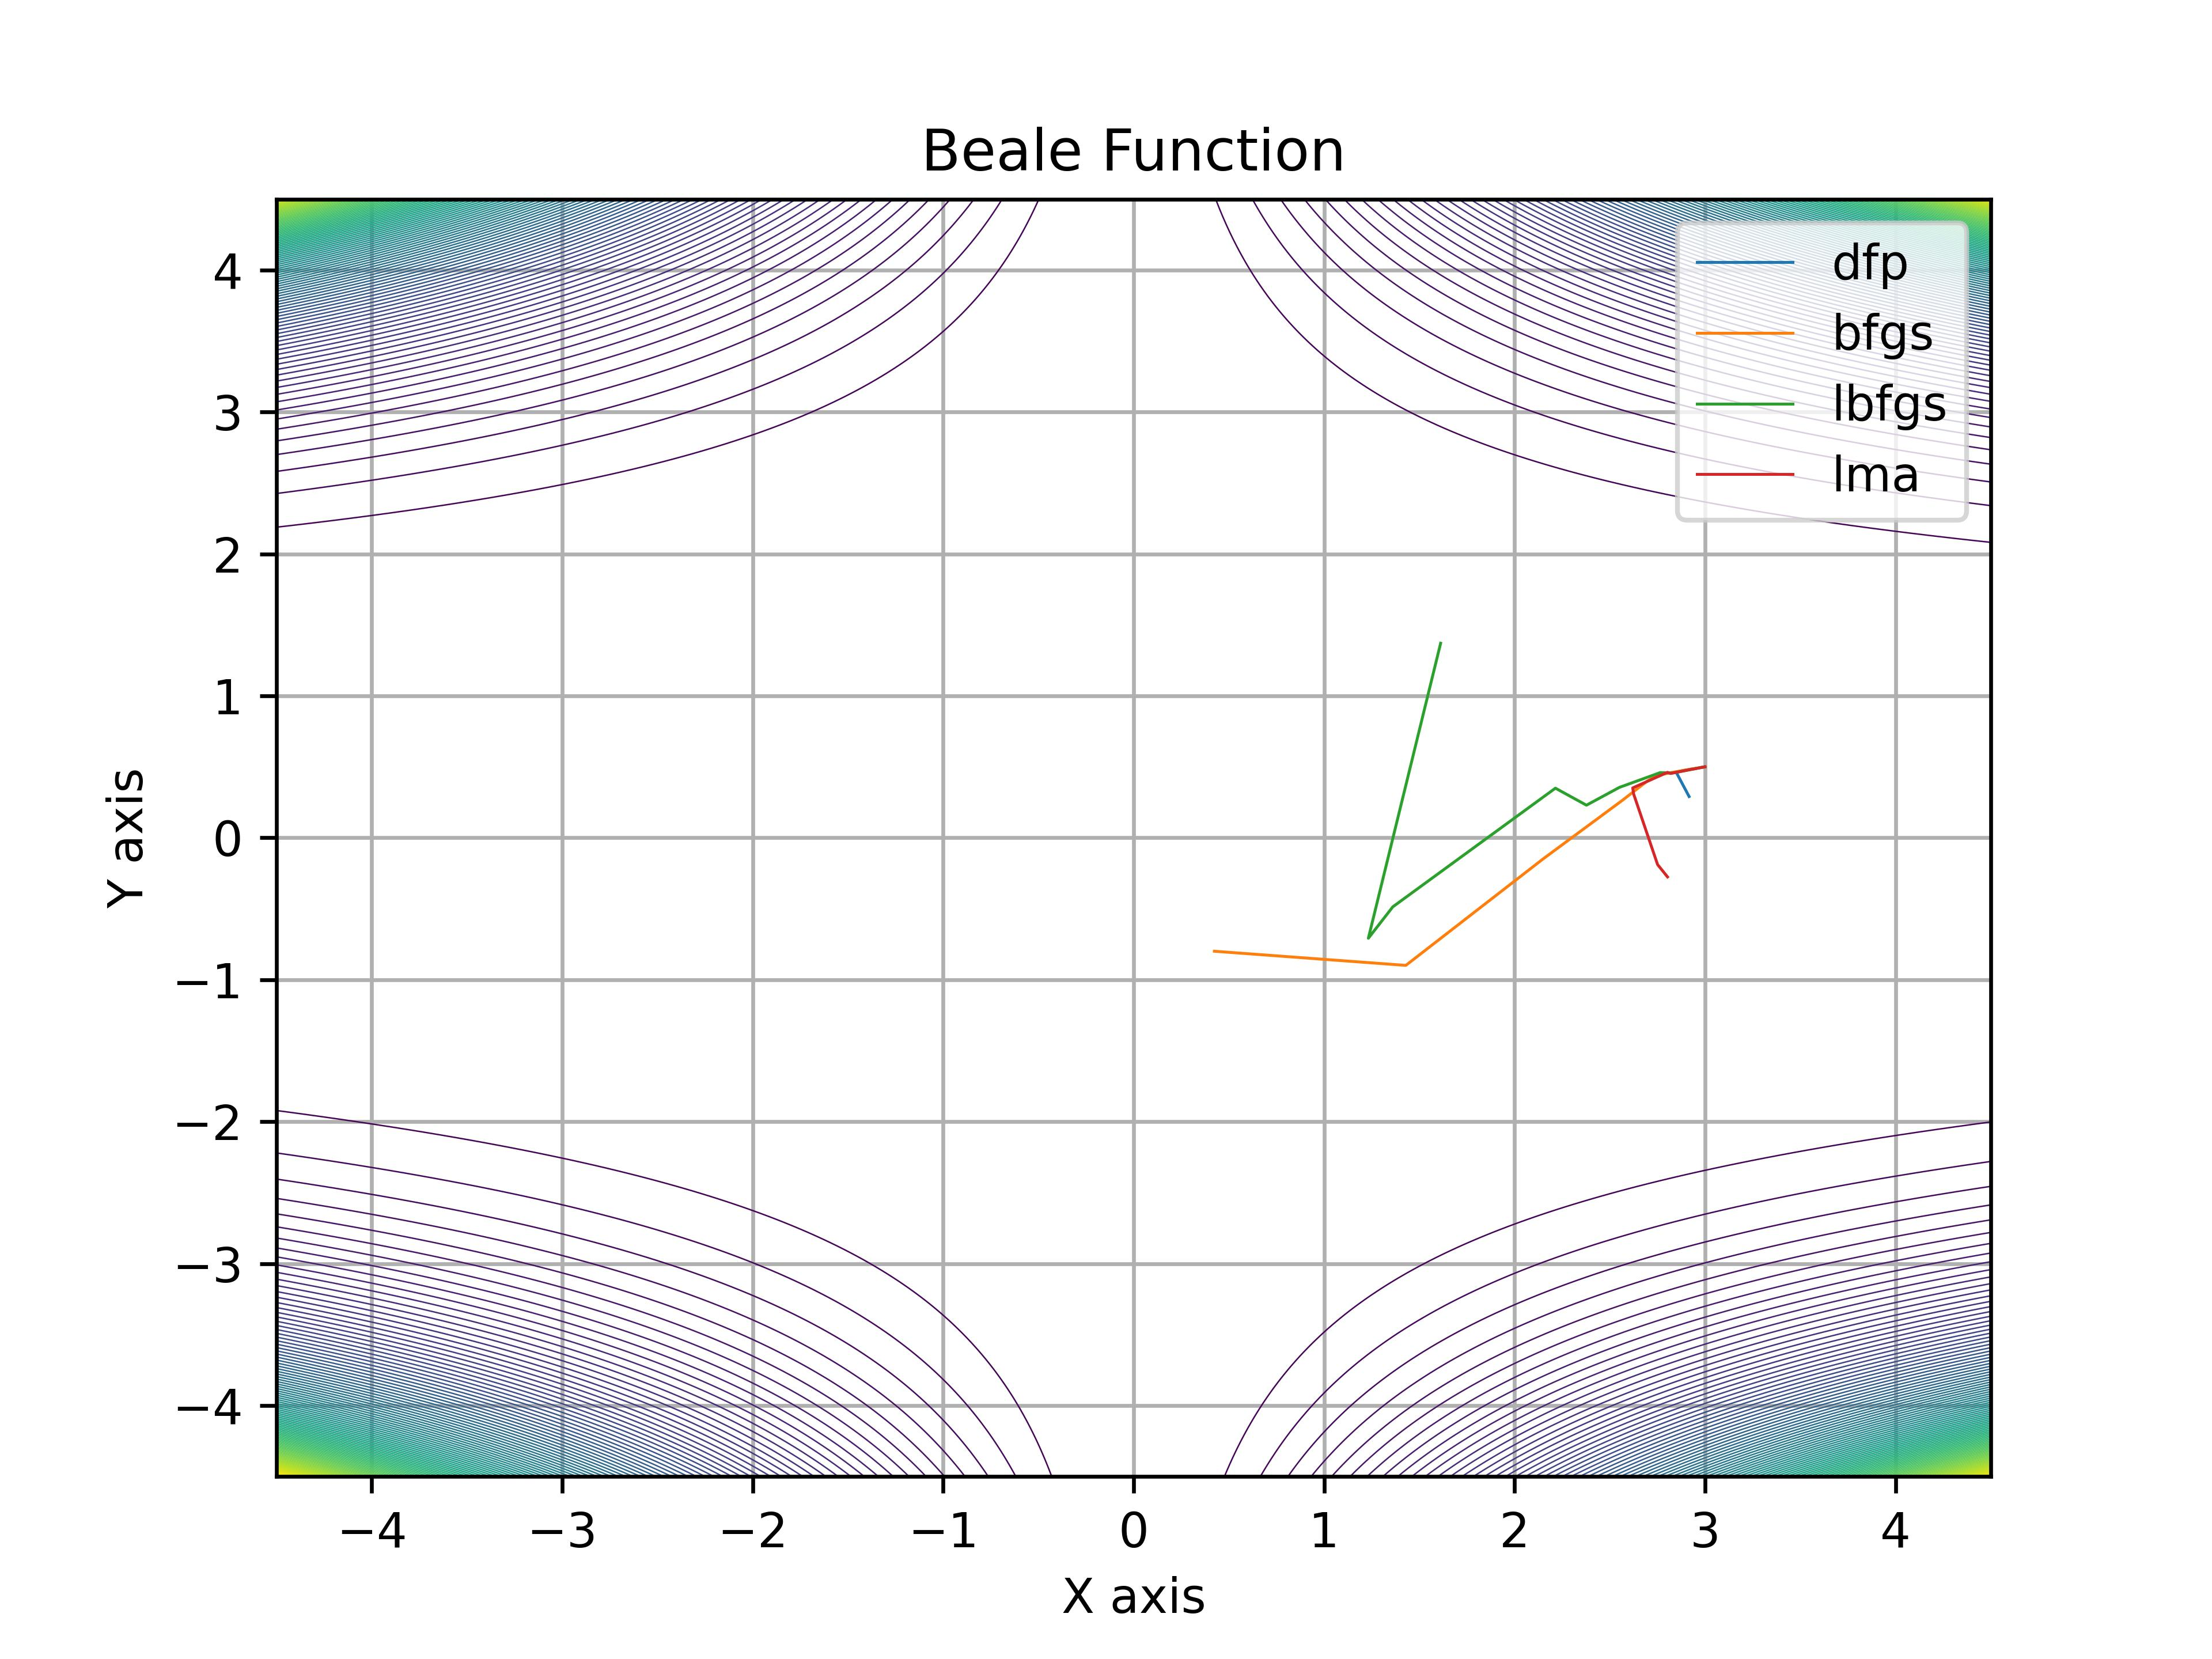
\includegraphics[scale=0.5]{images/beale.jpg}
\end{figure}
The isolines for Beale Function shows that there are a large plateau near the solution. For an unknown reason the best algorithm had 80\% of performance at its best. Quasi-Newton algorithms suffers to converge when the gradient is less significant.\subsection{Booth Function}
\label{booth2D}

\subsubsection{Convergence Analysis}
\label{convergencebooth2D}

\begin{table}[H]
\centering
\caption{Convergence Report For Booth Function}
\label{convergence:booth}
\begin{tabular}{lrrrr}
\toprule
 Alg. &  Good &  Poor &  Diver. &  Total \\
\midrule
  dfp &   100 &     0 &       0 &    100 \\
 bfgs &   100 &     0 &       0 &    100 \\
lbfgs &   100 &     0 &       0 &    100 \\
  lma &   100 &     0 &       0 &    100 \\
\bottomrule
\end{tabular}
\end{table}

\subsubsection{Statistical Analysis of The Solutions}
\label{statisticalanalysisbooth2D}

\begin{table}[H]
\centering
\caption{Statistical Information about function values For Booth Function}
\label{function_values:booth}
\begin{tabular}{lrrrr}
\toprule
 Alg. &  Min &  Max &  Mean &  Median \\
\midrule
  dfp & 0.00 & 0.00 &  0.00 &    0.00 \\
 bfgs & 0.00 & 0.00 &  0.00 &    0.00 \\
lbfgs & 0.00 & 0.00 &  0.00 &    0.00 \\
  lma & 0.00 & 0.00 &  0.00 &    0.00 \\
\bottomrule
\end{tabular}
\end{table}

\subsubsection{Best Fits}
\label{bestfitsbooth2D}

The best solutions of all algorithms for Booth Function, obtained using the minimal
distance of the solution, are shown in Table~\ref{solutions:booth}:
\begin{table}[H]
\centering
\caption{Best Fits For Booth Function}
\label{solutions:booth}
\begin{tabular}{llrrr}
\toprule
 Alg. &    Sol. &  Iter. &  F. Eval &  F. Value \\
\midrule
  dfp & $S_{1}$ &      4 &        6 &      0.00 \\
 bfgs & $S_{2}$ &      2 &        5 &      0.00 \\
lbfgs & $S_{3}$ &      5 &       21 &      0.00 \\
  lma & $S_{4}$ &     10 &       11 &      0.00 \\
\bottomrule
\end{tabular}
\end{table}



Altough the column F. Value points to the the same value, this is a rounded value
and the real values are os order $10^{-22} \approx 10^{-14}$.

\begin{table}[H]
\centering
\caption{Detailed Solutions For Booth Function}
\label{detailedsolutions:booth}
\begin{tabular}{lrrrr}
\toprule
 Coord. &  $S_{1}$ &  $S_{2}$ &  $S_{3}$ &  $S_{4}$ \\
\midrule
$x_{1}$ &     1.00 &     1.00 &     1.00 &     1.00 \\
$x_{2}$ &     3.00 &     3.00 &     3.00 &     3.00 \\
\bottomrule
\end{tabular}
\end{table}

\subsubsection{Isolines and Convergence line}
\label{isolinesbooth2D}

\begin{figure}[H]
\centering
\caption{Isolines and convergence line for Booth Function}
\label{fig:booth}
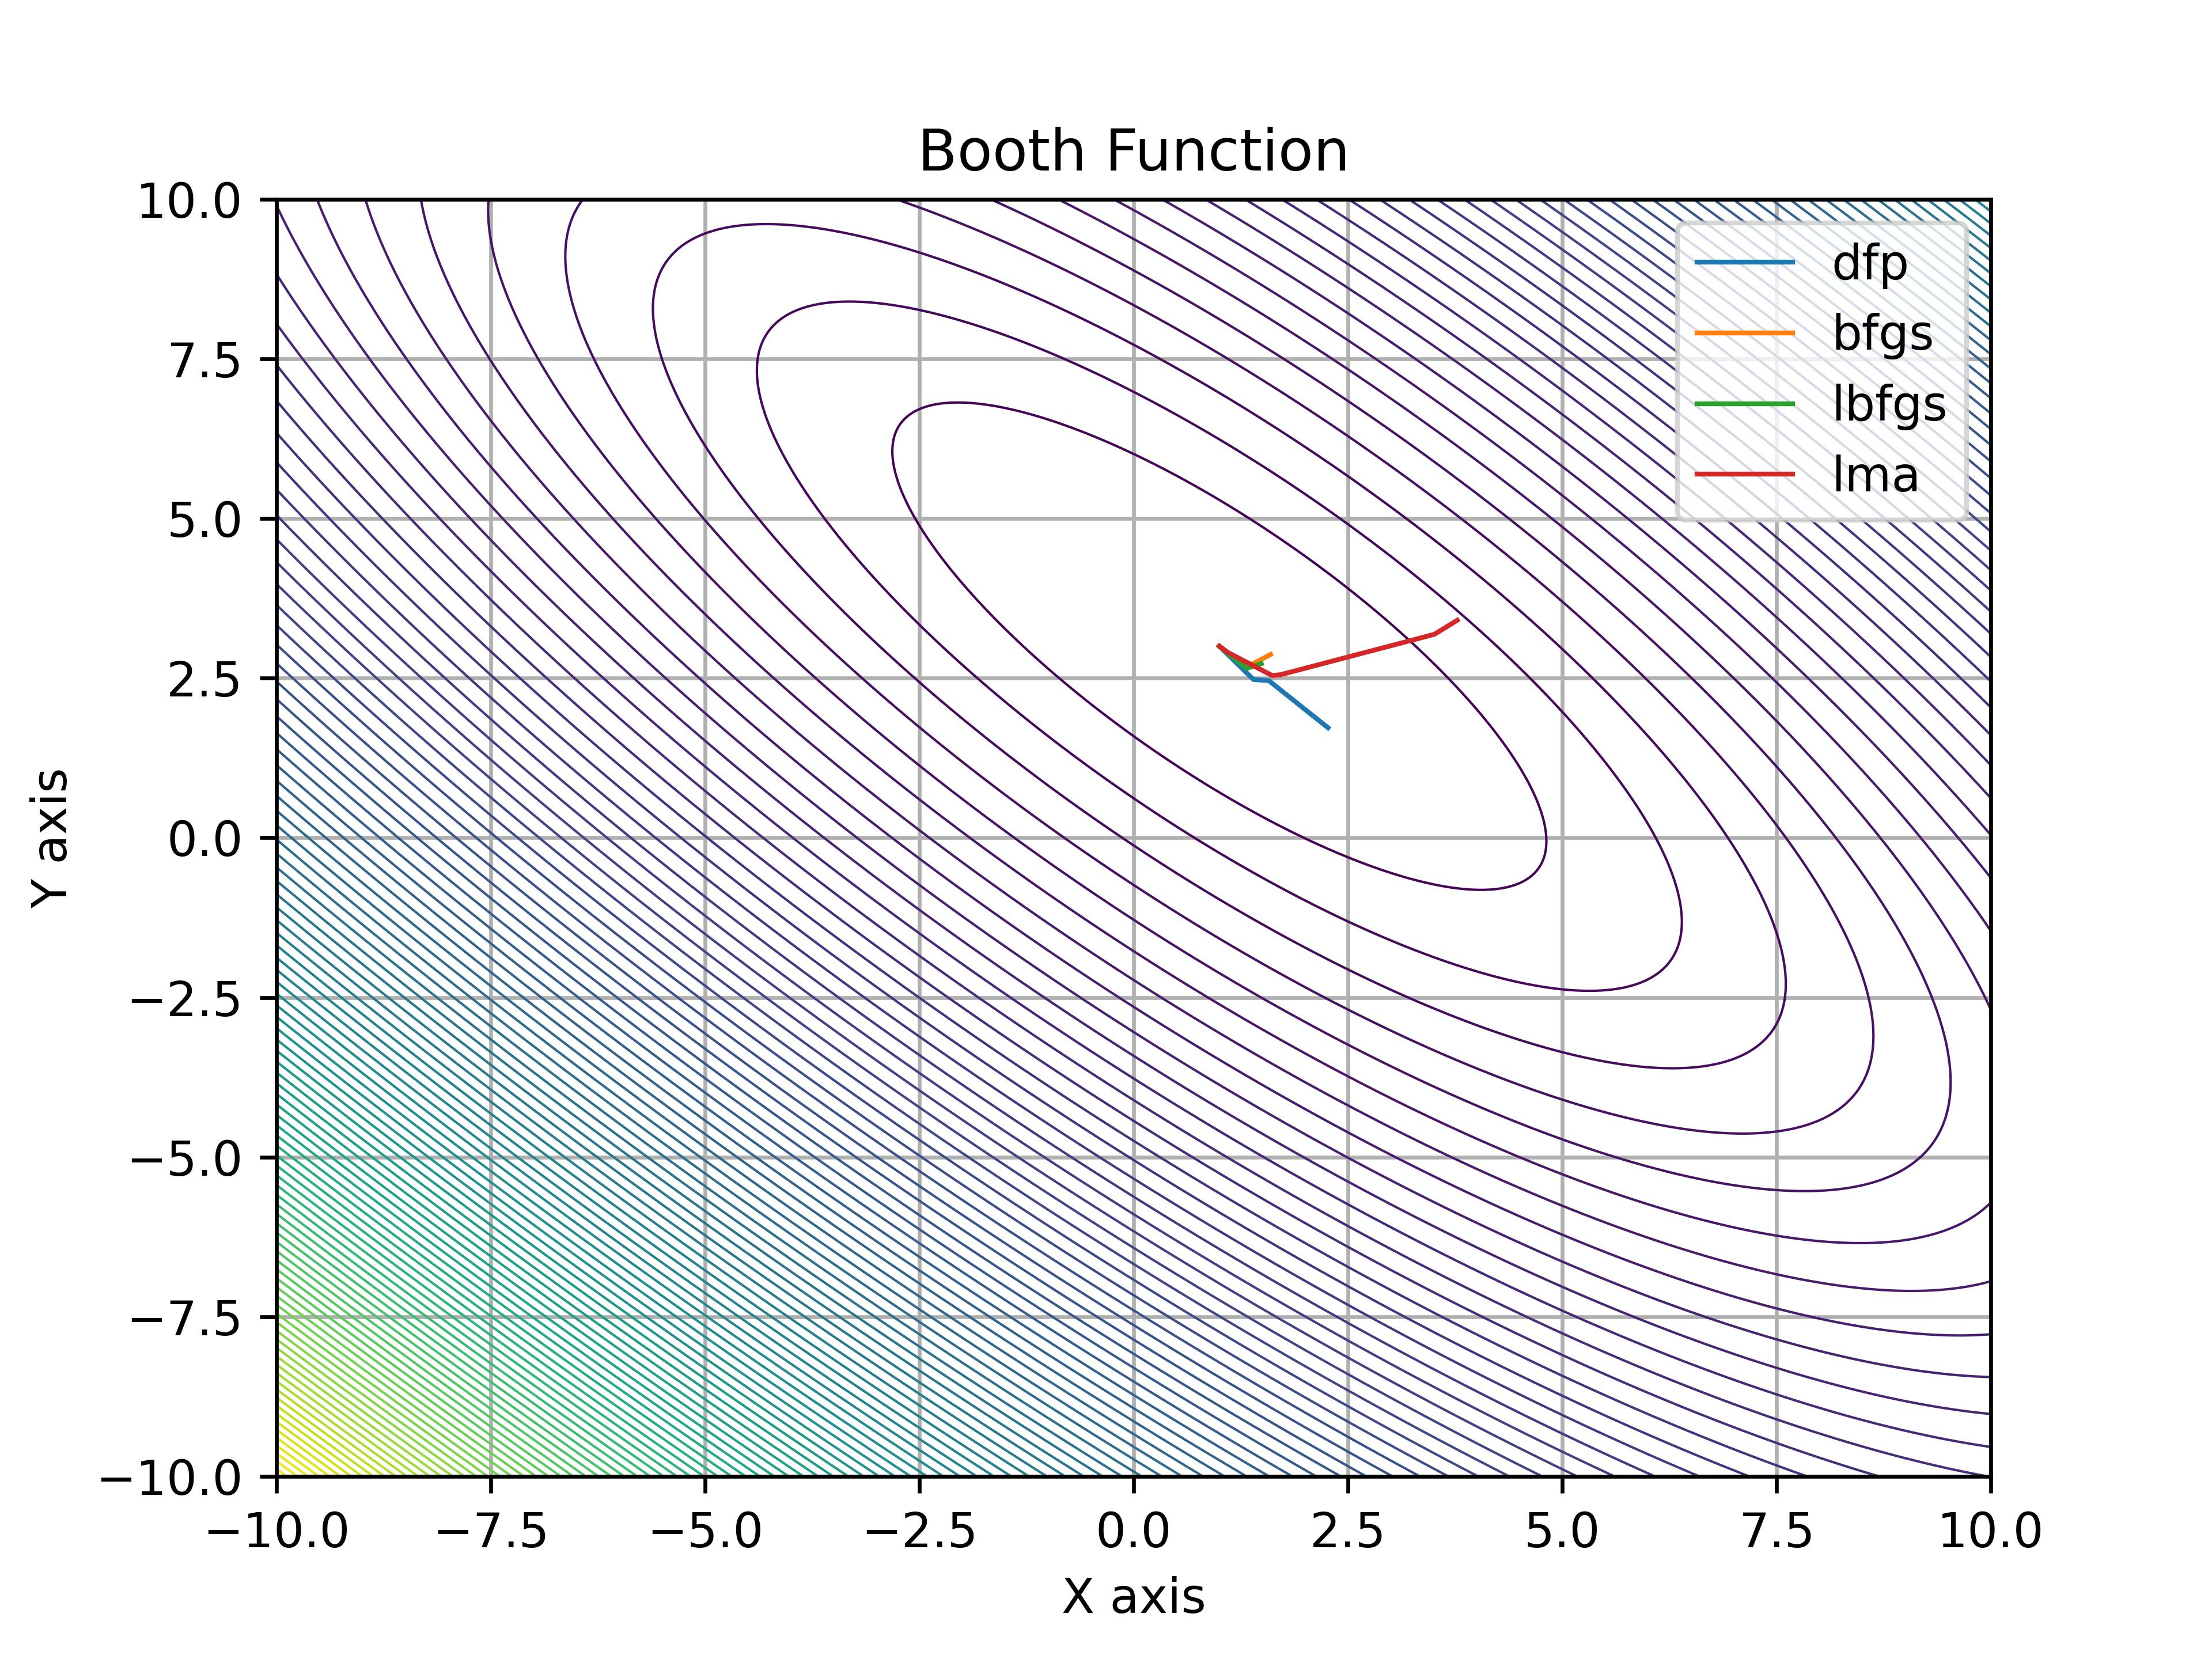
\includegraphics[scale=0.5]{images/booth.jpg}
\end{figure}
\subsection{Matyas Function}
\label{matyas2D}

\subsubsection{Convergence Analysis}
\label{convergencematyas2D}

\begin{table}[H]
\centering
\caption{Convergence Report For Matyas Function}
\label{convergence:matyas}
\begin{tabular}{lrrrr}
\toprule
 Alg. &  Good &  Poor &  Diver. &  Total \\
\midrule
  dfp &   100 &     0 &       0 &    100 \\
 bfgs &   100 &     0 &       0 &    100 \\
lbfgs &   100 &     0 &       0 &    100 \\
  lma &   100 &     0 &       0 &    100 \\
\bottomrule
\end{tabular}
\end{table}

\subsubsection{Statistical Analysis of The Solutions}
\label{statisticalanalysismatyas2D}

\begin{table}[H]
\centering
\caption{Statistical Information about function values For Matyas Function}
\label{function_values:matyas}
\begin{tabular}{lrrrr}
\toprule
 Alg. &  Min &  Max &  Mean &  Median \\
\midrule
  dfp & 0.00 & 0.00 &  0.00 &    0.00 \\
 bfgs & 0.00 & 0.00 &  0.00 &    0.00 \\
lbfgs & 0.00 & 0.00 &  0.00 &    0.00 \\
  lma & 0.00 & 0.00 &  0.00 &    0.00 \\
\bottomrule
\end{tabular}
\end{table}

\subsubsection{Best Fits}
\label{bestfitsmatyas2D}

\begin{table}[H]
\centering
\caption{Best Fits For Matyas Function}
\label{solutions:matyas}
\begin{tabular}{llrrr}
\toprule
 Alg. &    Sol. &  Iter. &  F. Eval &  F. Value \\
\midrule
  dfp & $S_{1}$ &      7 &       10 &      0.00 \\
 bfgs & $S_{2}$ &      7 &       10 &      0.00 \\
lbfgs & $S_{3}$ &      4 &       16 &      0.00 \\
  lma & $S_{4}$ &     14 &       15 &      0.00 \\
\bottomrule
\end{tabular}
\end{table}

\begin{table}[H]
\centering
\caption{Detailed Solutions For Matyas Function}
\label{detailedsolutions:matyas}
\begin{tabular}{lrrrr}
\toprule
 Coord. &  $S_{1}$ &  $S_{2}$ &  $S_{3}$ &  $S_{4}$ \\
\midrule
$x_{1}$ &     0.00 &    -0.00 &    -0.00 &     0.00 \\
$x_{2}$ &     0.00 &    -0.00 &     0.00 &     0.00 \\
\bottomrule
\end{tabular}
\end{table}

\subsubsection{Isolines and Convergence line}
\label{isolinesmatyas2D}

\begin{figure}[H]
\centering
\caption{Isolines and convergence line for Matyas Function}
\label{fig:matyas}
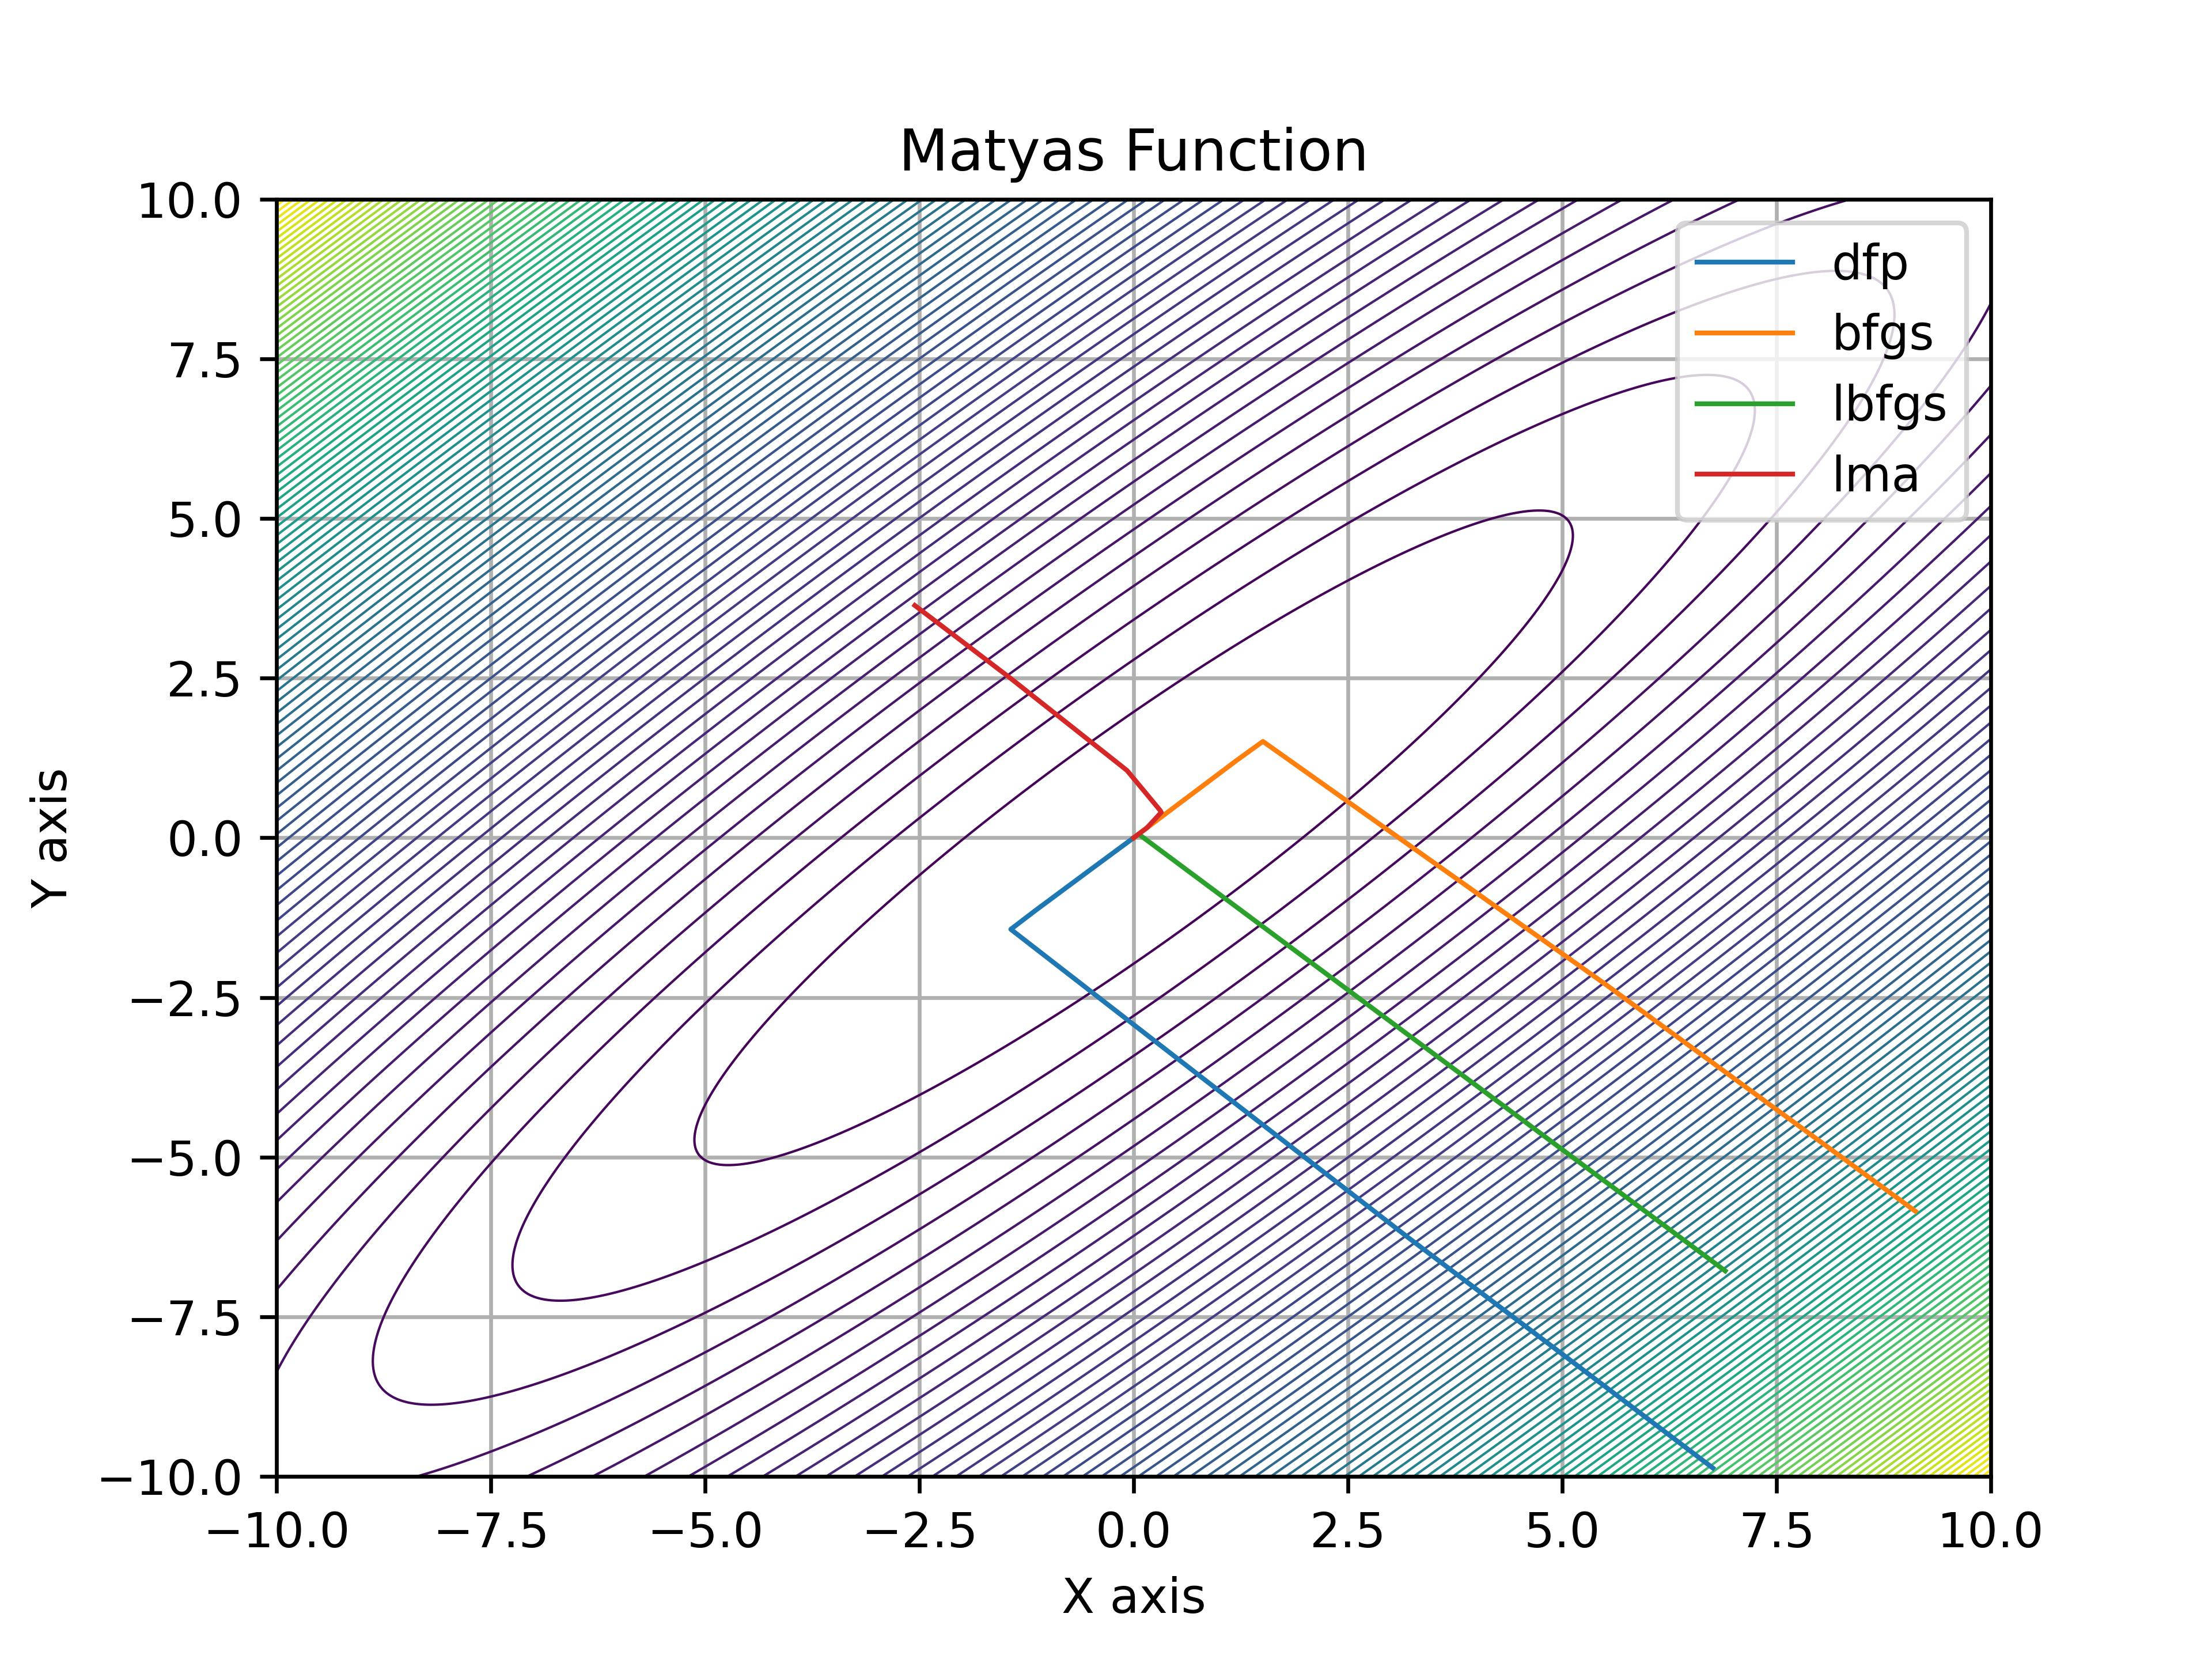
\includegraphics[scale=0.5]{images/matyas.jpg}
\end{figure}
\subsection{Rastrigin Function}
\label{rastrigin2d2D}

\subsubsection{Convergence Analysis}
\label{convergencerastrigin2d2D}

\begin{table}[H]
\centering
\caption{Convergence Report For Rastrigin Function}
\label{convergence:rastrigin2d}
\begin{tabular}{lrrrr}
\toprule
 Alg. &  Good &  Poor &  Diver. &  Total \\
\midrule
  dfp &   100 &     0 &       0 &    100 \\
 bfgs &   100 &     0 &       0 &    100 \\
lbfgs &    99 &     1 &       0 &    100 \\
  lma &   100 &     0 &       0 &    100 \\
\bottomrule
\end{tabular}
\end{table}

\subsubsection{Statistical Analysis of The Solutions}
\label{statisticalanalysisrastrigin2d2D}

\begin{table}[H]
\centering
\caption{Statistical Information about function values For Rastrigin Function}
\label{function_values:rastrigin2d}
\begin{tabular}{lrrrr}
\toprule
 Alg. &  Min &  Max &  Mean &  Median \\
\midrule
  dfp & 0.00 & 0.00 &  0.00 &    0.00 \\
 bfgs & 0.00 & 0.00 &  0.00 &    0.00 \\
lbfgs & 0.00 & 1.99 &  0.02 &    0.00 \\
  lma & 0.00 & 0.00 &  0.00 &    0.00 \\
\bottomrule
\end{tabular}
\end{table}

\subsubsection{Best Fits}
\label{bestfitsrastrigin2d2D}

\begin{table}[H]
\centering
\caption{Best Fits For Rastrigin Function}
\label{solutions:rastrigin2d}
\begin{tabular}{llrrr}
\toprule
 Alg. &    Sol. &  Iter. &  F. Eval &  F. Value \\
\midrule
  dfp & $S_{1}$ &      6 &       11 &      0.00 \\
 bfgs & $S_{2}$ &      8 &       49 &      0.00 \\
lbfgs & $S_{3}$ &      5 &      133 &      0.00 \\
  lma & $S_{4}$ &      4 &        5 &      0.00 \\
\bottomrule
\end{tabular}
\end{table}

\begin{table}[H]
\centering
\caption{Detailed Solutions For Rastrigin Function}
\label{detailedsolutions:rastrigin2d}
\begin{tabular}{lrrrr}
\toprule
 Coord. &  $S_{1}$ &  $S_{2}$ &  $S_{3}$ &  $S_{4}$ \\
\midrule
$x_{1}$ &    -0.00 &     0.00 &     0.00 &     0.00 \\
$x_{2}$ &     0.00 &    -0.00 &    -0.00 &     0.00 \\
\bottomrule
\end{tabular}
\end{table}

\subsubsection{Isolines and Convergence line}
\label{isolinesrastrigin2d2D}

\begin{figure}[H]
\centering
\caption{Isolines and convergence line for Rastrigin Function}
\label{fig:rastrigin2d}
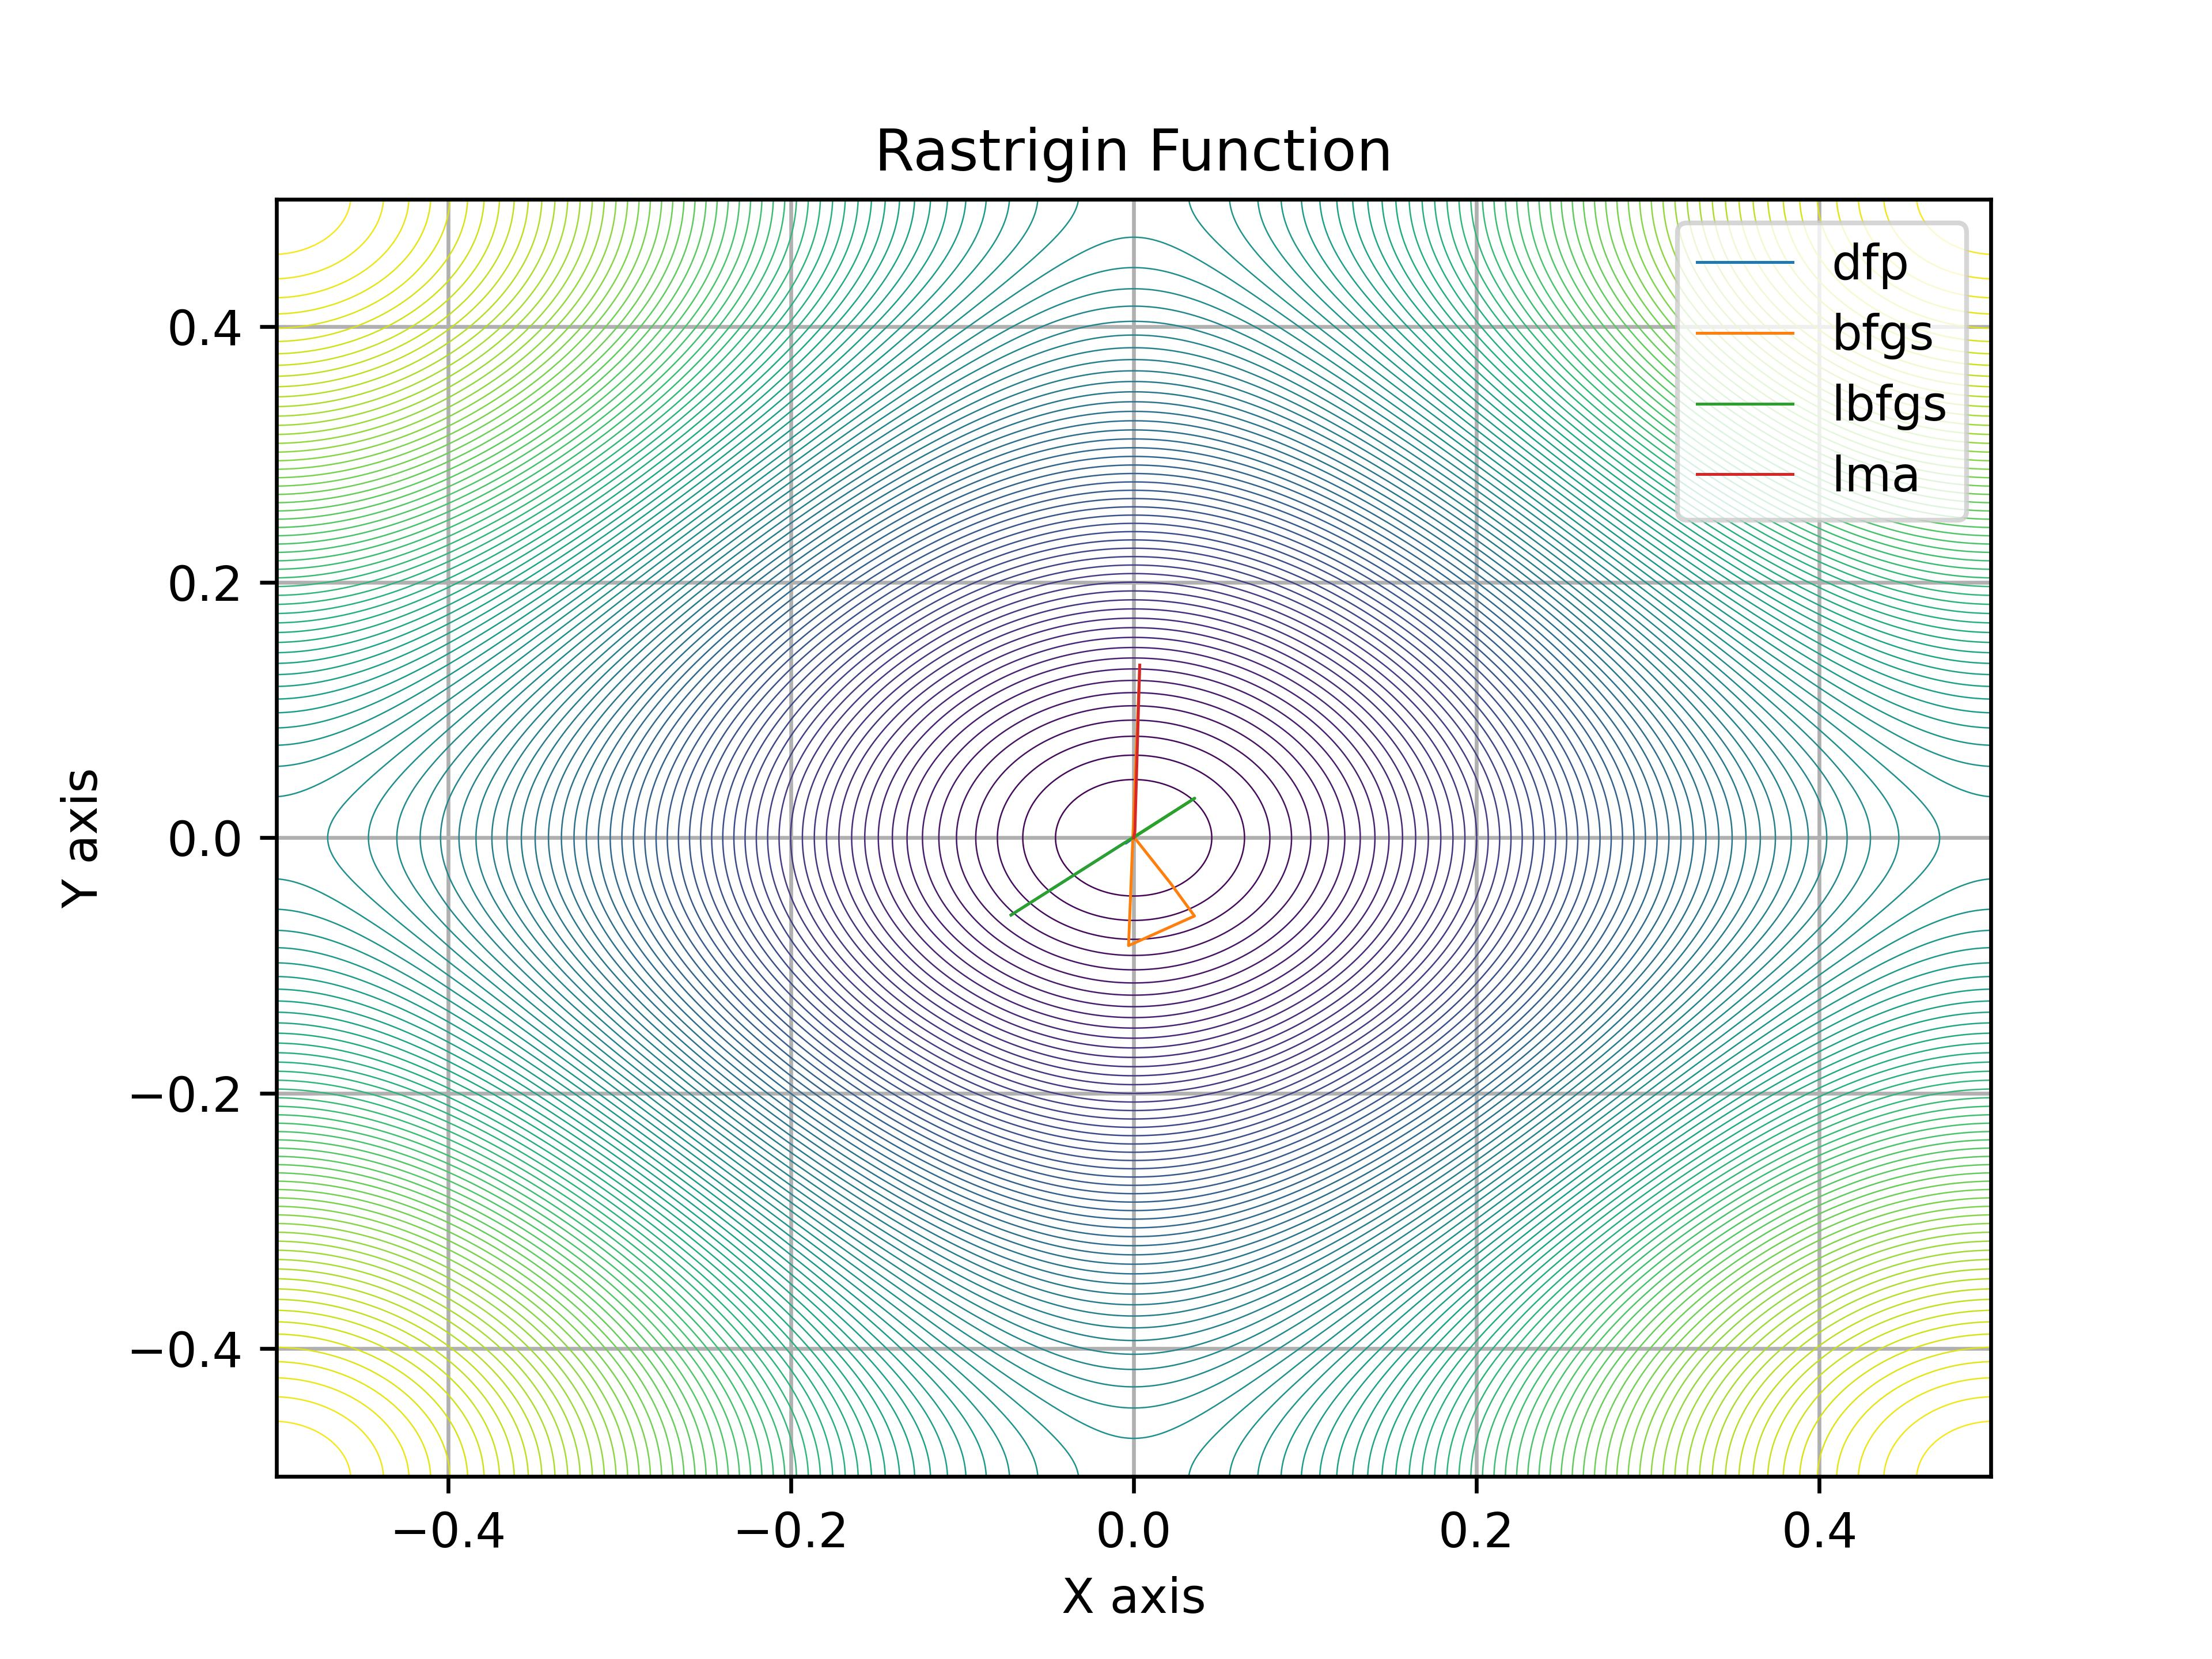
\includegraphics[scale=0.5]{images/rastrigin2d.jpg}
\end{figure}
\subsection{Rosenbrock Function}
\label{rosenbrock2d2D}

\subsubsection{Convergence Analysis}
\label{convergencerosenbrock2d2D}

\begin{table}[H]
\centering
\caption{Convergence Report For Rosenbrock Function}
\label{convergence:rosenbrock2d}
\begin{tabular}{lrrrr}
\toprule
 Alg. &  Good &  Poor &  Diver. &  Total \\
\midrule
  dfp &    74 &    26 &       0 &    100 \\
 bfgs &   100 &     0 &       0 &    100 \\
lbfgs &   100 &     0 &       0 &    100 \\
  lma &   100 &     0 &       0 &    100 \\
\bottomrule
\end{tabular}
\end{table}

\subsubsection{Statistical Analysis of The Solutions}
\label{statisticalanalysisrosenbrock2d2D}

\begin{table}[H]
\centering
\caption{Statistical Information about function values For Rosenbrock Function}
\label{function_values:rosenbrock2d}
\begin{tabular}{lrrrr}
\toprule
 Alg. &  Min &  Max &  Mean &  Median \\
\midrule
  dfp & 0.00 & 1.33 &  0.04 &    0.00 \\
 bfgs & 0.00 & 0.00 &  0.00 &    0.00 \\
lbfgs & 0.00 & 0.00 &  0.00 &    0.00 \\
  lma & 0.00 & 0.00 &  0.00 &    0.00 \\
\bottomrule
\end{tabular}
\end{table}

\subsubsection{Best Fits}
\label{bestfitsrosenbrock2d2D}

\begin{table}[H]
\centering
\caption{Best Fits For Rosenbrock Function}
\label{solutions:rosenbrock2d}
\begin{tabular}{llrrr}
\toprule
 Alg. &    Sol. &  Iter. &  F. Eval &  F. Value \\
\midrule
  dfp & $S_{1}$ &     24 &       31 &      0.00 \\
 bfgs & $S_{2}$ &     30 &       43 &      0.00 \\
lbfgs & $S_{3}$ &     27 &       76 &      0.00 \\
  lma & $S_{4}$ &     16 &       18 &      0.00 \\
\bottomrule
\end{tabular}
\end{table}

\begin{table}[H]
\centering
\caption{Detailed Solutions For Rosenbrock Function}
\label{detailedsolutions:rosenbrock2d}
\begin{tabular}{lrrrr}
\toprule
 Coord. &  $S_{1}$ &  $S_{2}$ &  $S_{3}$ &  $S_{4}$ \\
\midrule
$x_{1}$ &     1.00 &     1.00 &     1.00 &     1.00 \\
$x_{2}$ &     1.00 &     1.00 &     1.00 &     1.00 \\
\bottomrule
\end{tabular}
\end{table}

\subsubsection{Isolines and Convergence line}
\label{isolinesrosenbrock2d2D}

\begin{figure}[H]
\centering
\caption{Isolines and convergence line for Rosenbrock Function}
\label{fig:rosenbrock2d}
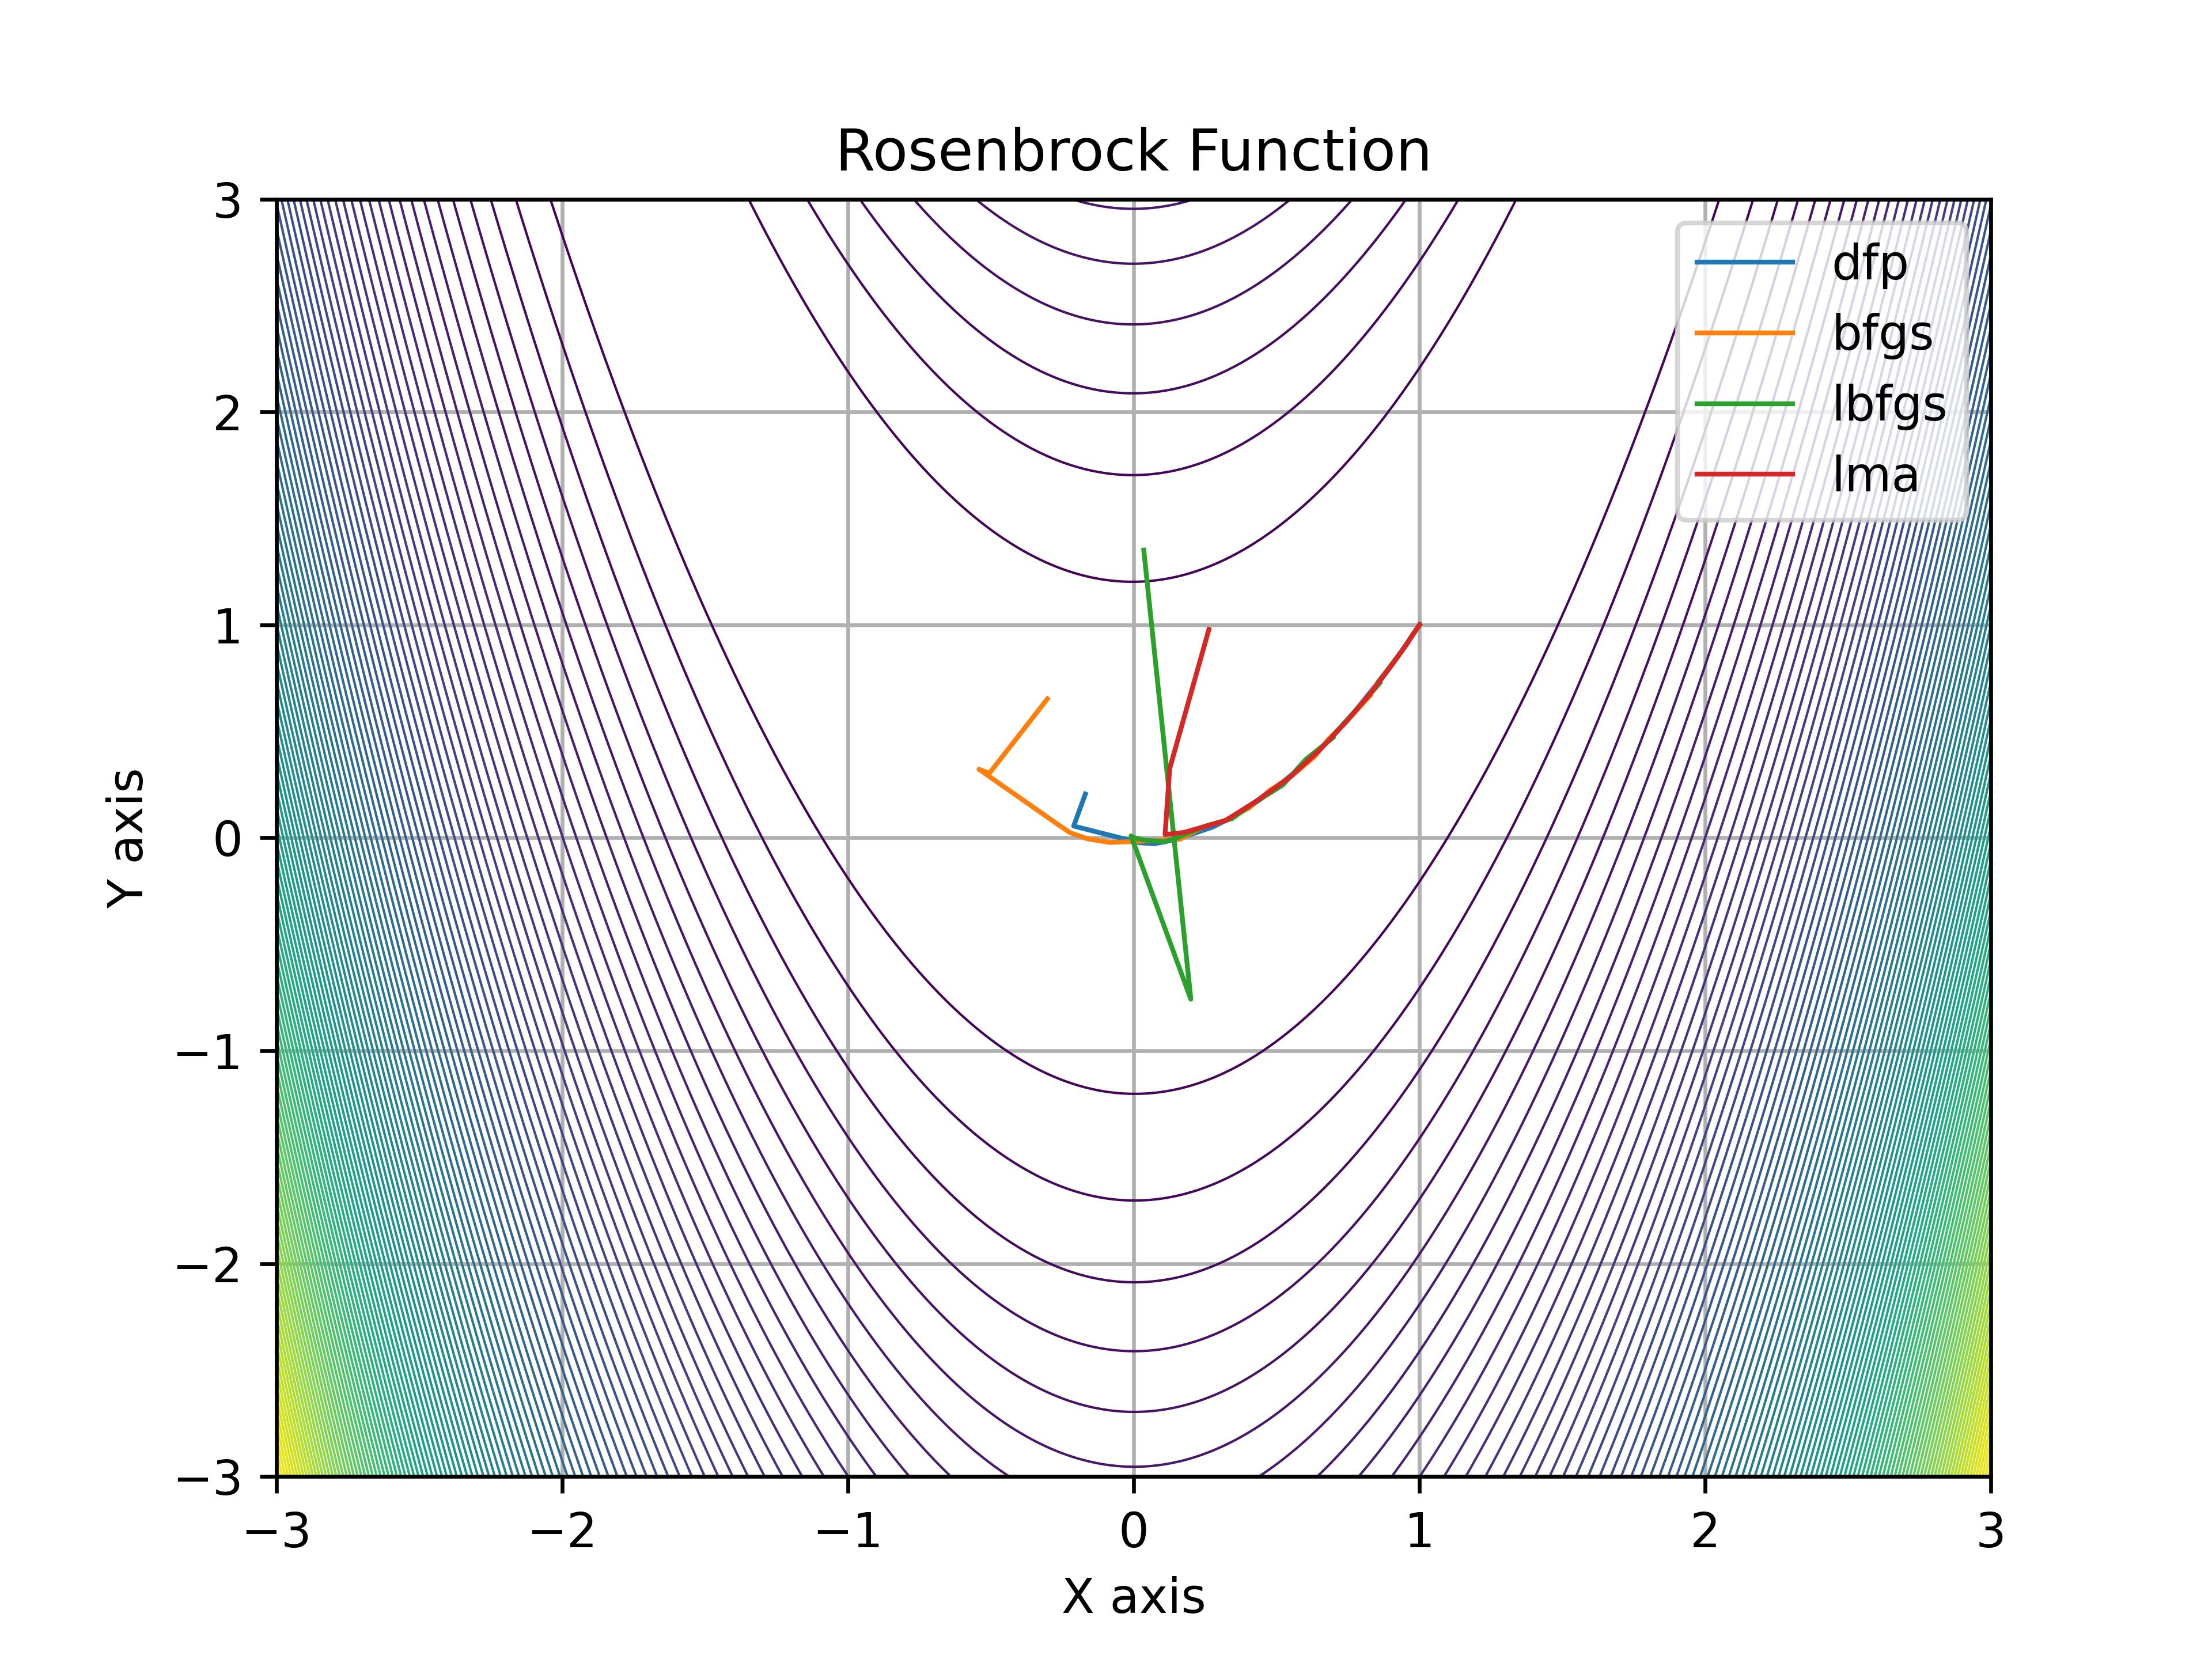
\includegraphics[scale=0.5]{images/rosenbrock2d.jpg}
\end{figure}

\section{4D Function versions}
\label{functions4D}

\subsection{Rastrigin Function}
\label{rastrigin4d4D}

\subsubsection{Convergence Analysis}
\label{convergencerastrigin4d4D}

\begin{table}[H]
\centering
\caption{Convergence Report For Rastrigin Function}
\label{convergence:rastrigin4d}
\begin{tabular}{lrrrr}
\toprule
 Alg. &  Good &  Poor &  Diver. &  Total \\
\midrule
  dfp &   100 &     0 &       0 &    100 \\
 bfgs &   100 &     0 &       0 &    100 \\
lbfgs &   100 &     0 &       0 &    100 \\
  lma &   100 &     0 &       0 &    100 \\
\bottomrule
\end{tabular}
\end{table}

\subsubsection{Statistical Analysis of The Solutions}
\label{statisticalanalysisrastrigin4d4D}

\begin{table}[H]
\centering
\caption{Statistical Information about function values For Rastrigin Function}
\label{function_values:rastrigin4d}
\begin{tabular}{lrrrr}
\toprule
 Alg. &  Min &  Max &  Mean &  Median \\
\midrule
  dfp & 0.00 & 0.00 &  0.00 &    0.00 \\
 bfgs & 0.00 & 0.00 &  0.00 &    0.00 \\
lbfgs & 0.00 & 0.00 &  0.00 &    0.00 \\
  lma & 0.00 & 0.00 &  0.00 &    0.00 \\
\bottomrule
\end{tabular}
\end{table}

\subsubsection{Best Fits}
\label{bestfitsrastrigin4d4D}

\begin{table}[H]
\centering
\caption{Best Fits For Rastrigin Function}
\label{solutions:rastrigin4d}
\begin{tabular}{llrrr}
\toprule
 Alg. &    Sol. &  Iter. &  F. Eval &  F. Value \\
\midrule
  dfp & $S_{1}$ &     10 &       21 &      0.00 \\
 bfgs & $S_{2}$ &     11 &       61 &      0.00 \\
lbfgs & $S_{3}$ &      5 &      133 &      0.00 \\
  lma & $S_{4}$ &      4 &        5 &      0.00 \\
\bottomrule
\end{tabular}
\end{table}

\begin{table}[H]
\centering
\caption{Detailed Solutions For Rastrigin Function}
\label{detailedsolutions:rastrigin4d}
\begin{tabular}{lrrrr}
\toprule
 Coord. &  $S_{1}$ &  $S_{2}$ &  $S_{3}$ &  $S_{4}$ \\
\midrule
$x_{1}$ &     0.00 &     0.00 &     0.00 &     0.00 \\
$x_{2}$ &    -0.00 &    -0.00 &     0.00 &     0.00 \\
$x_{3}$ &    -0.00 &    -0.00 &     0.00 &    -0.00 \\
$x_{4}$ &    -0.00 &    -0.00 &     0.00 &     0.00 \\
\bottomrule
\end{tabular}
\end{table}

\subsection{Rosenbrock Function}
\label{rosenbrock4d4D}

\subsubsection{Convergence Analysis}
\label{convergencerosenbrock4d4D}

\begin{table}[H]
\centering
\caption{Convergence Report For Rosenbrock Function}
\label{convergence:rosenbrock4d}
\begin{tabular}{lrrrr}
\toprule
 Alg. &  Good &  Poor &  Diver. &  Total \\
\midrule
  dfp &    46 &    54 &       0 &    100 \\
 bfgs &    90 &    10 &       0 &    100 \\
lbfgs &    89 &    11 &       0 &    100 \\
  lma &    91 &     9 &       0 &    100 \\
\bottomrule
\end{tabular}
\end{table}

\subsubsection{Statistical Analysis of The Solutions}
\label{statisticalanalysisrosenbrock4d4D}

\begin{table}[H]
\centering
\caption{Statistical Information about function values For Rosenbrock Function}
\label{function_values:rosenbrock4d}
\begin{tabular}{lrrrr}
\toprule
 Alg. &  Min &  Max &  Mean &  Median \\
\midrule
  dfp & 0.00 & 3.71 &  0.60 &    0.00 \\
 bfgs & 0.00 & 3.70 &  0.37 &    0.00 \\
lbfgs & 0.00 & 3.70 &  0.41 &    0.00 \\
  lma & 0.00 & 3.70 &  0.33 &    0.00 \\
\bottomrule
\end{tabular}
\end{table}

\subsubsection{Best Fits}
\label{bestfitsrosenbrock4d4D}

\begin{table}[H]
\centering
\caption{Best Fits For Rosenbrock Function}
\label{solutions:rosenbrock4d}
\begin{tabular}{llrrr}
\toprule
 Alg. &    Sol. &  Iter. &  F. Eval &  F. Value \\
\midrule
  dfp & $S_{1}$ &     44 &       49 &      0.00 \\
 bfgs & $S_{2}$ &     29 &       35 &      0.00 \\
lbfgs & $S_{3}$ &     45 &      134 &      0.00 \\
  lma & $S_{4}$ &     18 &       20 &      0.00 \\
\bottomrule
\end{tabular}
\end{table}

\begin{table}[H]
\centering
\caption{Detailed Solutions For Rosenbrock Function}
\label{detailedsolutions:rosenbrock4d}
\begin{tabular}{lrrrr}
\toprule
 Coord. &  $S_{1}$ &  $S_{2}$ &  $S_{3}$ &  $S_{4}$ \\
\midrule
$x_{1}$ &     1.00 &     1.00 &     1.00 &     1.00 \\
$x_{2}$ &     1.00 &     1.00 &     1.00 &     1.00 \\
$x_{3}$ &     1.00 &     1.00 &     1.00 &     1.00 \\
$x_{4}$ &     1.00 &     1.00 &     1.00 &     1.00 \\
\bottomrule
\end{tabular}
\end{table}


\section{30D Function versions}
\label{functions30D}

\subsection{Rastrigin Function}
\label{rastrigin30d30D}

\subsubsection{Convergence Analysis}
\label{convergencerastrigin30d30D}

\begin{table}[H]
\centering
\caption{Convergence Report For Rastrigin Function}
\label{convergence:rastrigin30d}
\begin{tabular}{lrrrr}
\toprule
 Alg. &  Good &  Poor &  Diver. &  Total \\
\midrule
  dfp &   100 &     0 &       0 &    100 \\
 bfgs &   100 &     0 &       0 &    100 \\
lbfgs &   100 &     0 &       0 &    100 \\
  lma &   100 &     0 &       0 &    100 \\
\bottomrule
\end{tabular}
\end{table}

\subsubsection{Statistical Analysis of The Solutions}
\label{statisticalanalysisrastrigin30d30D}

\begin{table}[H]
\centering
\caption{Statistical Information about function values For Rastrigin Function}
\label{function_values:rastrigin30d}
\begin{tabular}{lrrrr}
\toprule
 Alg. &  Min &  Max &  Mean &  Median \\
\midrule
  dfp & 0.00 & 0.00 &  0.00 &    0.00 \\
 bfgs & 0.00 & 0.00 &  0.00 &    0.00 \\
lbfgs & 0.00 & 0.00 &  0.00 &    0.00 \\
  lma & 0.00 & 0.00 &  0.00 &    0.00 \\
\bottomrule
\end{tabular}
\end{table}

\subsubsection{Best Fits}
\label{bestfitsrastrigin30d30D}

\begin{table}[H]
\centering
\caption{Best Fits For Rastrigin Function}
\label{solutions:rastrigin30d}
\begin{tabular}{llrrr}
\toprule
 Alg. &    Sol. &  Iter. &  F. Eval &  F. Value \\
\midrule
  dfp & $S_{1}$ &      8 &       14 &      0.00 \\
 bfgs & $S_{2}$ &      9 &       54 &      0.00 \\
lbfgs & $S_{3}$ &      6 &      135 &      0.00 \\
  lma & $S_{4}$ &      4 &        5 &      0.00 \\
\bottomrule
\end{tabular}
\end{table}

\begin{table}[H]
\centering
\caption{Detailed Solutions For Rastrigin Function}
\label{detailedsolutions:rastrigin30d}
\begin{tabular}{lrrrr}
\toprule
  Coord. &  $S_{1}$ &  $S_{2}$ &  $S_{3}$ &  $S_{4}$ \\
\midrule
 $x_{1}$ &    -0.00 &     0.00 &     0.00 &     0.00 \\
 $x_{2}$ &    -0.00 &     0.00 &     0.00 &     0.00 \\
 $x_{3}$ &    -0.00 &     0.00 &    -0.00 &    -0.00 \\
 $x_{4}$ &    -0.00 &     0.00 &     0.00 &     0.00 \\
 $x_{5}$ &     0.00 &    -0.00 &    -0.00 &    -0.00 \\
 $x_{6}$ &     0.00 &    -0.00 &    -0.00 &    -0.00 \\
 $x_{7}$ &     0.00 &    -0.00 &     0.00 &     0.00 \\
 $x_{8}$ &     0.00 &    -0.00 &    -0.00 &    -0.00 \\
 $x_{9}$ &    -0.00 &     0.00 &     0.00 &     0.00 \\
$x_{10}$ &    -0.00 &     0.00 &     0.00 &    -0.00 \\
$x_{11}$ &     0.00 &    -0.00 &     0.00 &     0.00 \\
$x_{12}$ &    -0.00 &     0.00 &     0.00 &     0.00 \\
$x_{13}$ &     0.00 &    -0.00 &    -0.00 &    -0.00 \\
$x_{14}$ &     0.00 &    -0.00 &     0.00 &     0.00 \\
$x_{15}$ &     0.00 &    -0.00 &    -0.00 &    -0.00 \\
$x_{16}$ &     0.00 &    -0.00 &    -0.00 &    -0.00 \\
$x_{17}$ &    -0.00 &     0.00 &    -0.00 &    -0.00 \\
$x_{18}$ &     0.00 &    -0.00 &    -0.00 &    -0.00 \\
$x_{19}$ &    -0.00 &     0.00 &    -0.00 &    -0.00 \\
$x_{20}$ &    -0.00 &     0.00 &    -0.00 &    -0.00 \\
$x_{21}$ &     0.00 &    -0.00 &     0.00 &     0.00 \\
$x_{22}$ &    -0.00 &     0.00 &    -0.00 &    -0.00 \\
$x_{23}$ &     0.00 &    -0.00 &    -0.00 &    -0.00 \\
$x_{24}$ &    -0.00 &     0.00 &    -0.00 &     0.00 \\
$x_{25}$ &    -0.00 &     0.00 &    -0.00 &     0.00 \\
$x_{26}$ &     0.00 &    -0.00 &     0.00 &     0.00 \\
$x_{27}$ &    -0.00 &     0.00 &     0.00 &     0.00 \\
$x_{28}$ &    -0.00 &     0.00 &    -0.00 &    -0.00 \\
$x_{29}$ &    -0.00 &     0.00 &    -0.00 &    -0.00 \\
$x_{30}$ &     0.00 &    -0.00 &    -0.00 &     0.00 \\
\bottomrule
\end{tabular}
\end{table}

\subsection{Rosenbrock Function}
\label{rosenbrock30d30D}

\subsubsection{Convergence Analysis}
\label{convergencerosenbrock30d30D}

\begin{table}[H]
\centering
\caption{Convergence Report For Rosenbrock Function}
\label{convergence:rosenbrock30d}
\begin{tabular}{lrrrr}
\toprule
 Alg. &  Good &  Poor &  Diver. &  Total \\
\midrule
  dfp &     1 &    99 &       0 &    100 \\
 bfgs &    80 &    20 &       0 &    100 \\
lbfgs &    95 &     5 &       0 &    100 \\
  lma &    88 &    12 &       0 &    100 \\
\bottomrule
\end{tabular}
\end{table}

\subsubsection{Statistical Analysis of The Solutions}
\label{statisticalanalysisrosenbrock30d30D}

\begin{table}[H]
\centering
\caption{Statistical Information about function values For Rosenbrock Function}
\label{function_values:rosenbrock30d}
\begin{tabular}{lrrrr}
\toprule
 Alg. &  Min &   Max &  Mean &  Median \\
\midrule
  dfp & 0.00 & 29.25 & 13.10 &   12.58 \\
 bfgs & 0.00 &  3.99 &  0.80 &    0.00 \\
lbfgs & 0.00 &  3.99 &  0.20 &    0.00 \\
  lma & 0.00 &  3.99 &  0.48 &    0.00 \\
\bottomrule
\end{tabular}
\end{table}

\subsubsection{Best Fits}
\label{bestfitsrosenbrock30d30D}

\begin{table}[H]
\centering
\caption{Best Fits For Rosenbrock Function}
\label{solutions:rosenbrock30d}
\begin{tabular}{llrrr}
\toprule
 Alg. &    Sol. &  Iter. &  F. Eval &  F. Value \\
\midrule
  dfp & $S_{1}$ &   2967 &     2990 &      0.00 \\
 bfgs & $S_{2}$ &    236 &      252 &      0.00 \\
lbfgs & $S_{3}$ &    164 &      406 &      0.00 \\
  lma & $S_{4}$ &     53 &      131 &      0.00 \\
\bottomrule
\end{tabular}
\end{table}

\begin{table}[H]
\centering
\caption{Detailed Solutions For Rosenbrock Function}
\label{detailedsolutions:rosenbrock30d}
\begin{tabular}{lrrrr}
\toprule
  Coord. &  $S_{1}$ &  $S_{2}$ &  $S_{3}$ &  $S_{4}$ \\
\midrule
 $x_{1}$ &     1.00 &     1.00 &     1.00 &     1.00 \\
 $x_{2}$ &     1.00 &     1.00 &     1.00 &     1.00 \\
 $x_{3}$ &     1.00 &     1.00 &     1.00 &     1.00 \\
 $x_{4}$ &     1.00 &     1.00 &     1.00 &     1.00 \\
 $x_{5}$ &     1.00 &     1.00 &     1.00 &     1.00 \\
 $x_{6}$ &     1.00 &     1.00 &     1.00 &     1.00 \\
 $x_{7}$ &     1.00 &     1.00 &     1.00 &     1.00 \\
 $x_{8}$ &     1.00 &     1.00 &     1.00 &     1.00 \\
 $x_{9}$ &     1.00 &     1.00 &     1.00 &     1.00 \\
$x_{10}$ &     1.00 &     1.00 &     1.00 &     1.00 \\
$x_{11}$ &     1.00 &     1.00 &     1.00 &     1.00 \\
$x_{12}$ &     1.00 &     1.00 &     1.00 &     1.00 \\
$x_{13}$ &     1.00 &     1.00 &     1.00 &     1.00 \\
$x_{14}$ &     1.00 &     1.00 &     1.00 &     1.00 \\
$x_{15}$ &     1.00 &     1.00 &     1.00 &     1.00 \\
$x_{16}$ &     1.00 &     1.00 &     1.00 &     1.00 \\
$x_{17}$ &     1.00 &     1.00 &     1.00 &     1.00 \\
$x_{18}$ &     1.00 &     1.00 &     1.00 &     1.00 \\
$x_{19}$ &     1.00 &     1.00 &     1.00 &     1.00 \\
$x_{20}$ &     1.00 &     1.00 &     1.00 &     1.00 \\
$x_{21}$ &     1.00 &     1.00 &     1.00 &     1.00 \\
$x_{22}$ &     1.00 &     1.00 &     1.00 &     1.00 \\
$x_{23}$ &     1.00 &     1.00 &     1.00 &     1.00 \\
$x_{24}$ &     1.00 &     1.00 &     1.00 &     1.00 \\
$x_{25}$ &     1.00 &     1.00 &     1.00 &     1.00 \\
$x_{26}$ &     1.00 &     1.00 &     1.00 &     1.00 \\
$x_{27}$ &     1.00 &     1.00 &     1.00 &     1.00 \\
$x_{28}$ &     1.00 &     1.00 &     1.00 &     1.00 \\
$x_{29}$ &     1.00 &     1.00 &     1.00 &     1.00 \\
$x_{30}$ &     1.00 &     1.00 &     1.00 &     1.00 \\
\bottomrule
\end{tabular}
\end{table}



\end{document}